% T12 C/D, chapitre 6 : Applications affines et isométries. Leçon : le livre « Terminales scientifiques » (Affine/Lesona, Isometrie/Lesona).
% Exercices et corrigés : originaux, écrits en novembre 2026 (les exercices tirés d’autres ouvrages ne sont pas repris, décision du 2 novembre 2026).

\TCDLessonStyleOn
\providecommand{\Plan}{\mathscr{P}}
\providecommand{\Espace}{\mathcal{E}}
\providecommand{\bary}[1]{\mathrm{Bar}\left\lbrace #1 \right\rbrace}
\providecommand{\Id}{\mathrm{Id}}
\chapter{Applications affines et isom\'etries}
      Dans ce chapitre, $\Plan$ d\'esigne le plan affine et $\Espace$ l'espace affine.
      \section{D\'efinitions et exemples}
            \begin{defi}
\index{Application affine}
                  Une application $f : \Plan \rightarrow \Plan$ est une \emph{application affine}
                  si elle conserve le barycentre.
                  
                  Si $G = \bary{(A,\alpha) ; (B,\beta)}$.
                  En posant $G' = f(G)$, $A' = f(A)$ et $B' = f(B)$, on a 
                  $G' = \bary{(A',\alpha) ; (B',\beta)}$.
            \end{defi}
            %
            \begin{ex}
                  \begin{enumerate}
                        \item Consid\'erons la translation $t_{\vec{u}}$ de vecteur $\vec{u}$.
                              En posant $t_{\vec{u}} (M) = M'$, on a $\overrightarrow{MM'} = \vec{u}$.
                              
                              Soit $G = \bary{(A,\alpha) ; (B,\beta)}$.
                              Soient
                              $G' = t_{\vec{u}} (G)$,
                              $A' = t_{\vec{u}} (A)$ et
                              $B' = t_{\vec{u}} (B)$
                              .
                              On a alors
                              \begin{align*}
                              \alpha \overrightarrow{G'A'} + \beta \overrightarrow{G'B'}
                                    & =  \alpha (\overrightarrow{G'G} + \overrightarrow{GA} + \overrightarrow{AA'})
                                        +\beta (\overrightarrow{G'G} + \overrightarrow{GB} + \overrightarrow{BB'})      \\
                                    & =  \alpha (-\vec{u} + \overrightarrow{GA} + \vec{u})
                                        +\beta (-\vec{u} + \overrightarrow{GB} + \vec{u})      \\
                                    & = \alpha \overrightarrow{GA} + \beta \overrightarrow{GB}      \\
                                    & = \vec{0}.
                              \end{align*}
                              Donc $G' = \bary{(A';\alpha);(B';\beta)}$ et ainsi, $t_{\vec{u}}$ est une application affine.
                  \end{enumerate}
            \end{ex}
            %
            \begin{ex}
                  Consid\'erons l'homoth\'etie $h$ de centre $I$ et de rapport $k$.
                  En posant $h(M) = M'$, on a $\overrightarrow{IM'} = k \overrightarrow{IM}$.
                  
                  On veut montrer que $h$ est une application affine.
                  Consid\'erons le point
                  \[
                  G = \bary{(A,\alpha);(B,\beta)}.
                  \]
                  Posons $G' = h(G)$, $A' = h(A)$ et $B' = h(B)$.
                  On a alors 
                  \begin{align*}
                        \alpha \overrightarrow{G'A'} + \beta \overrightarrow{G'B'}
                              & =  \alpha (\overrightarrow{G'I} + \overrightarrow{IA'})
                                  +\beta (\overrightarrow{G'I} + \overrightarrow{IB'})      \\
                              & = \alpha (k \overrightarrow{GI} + k \overrightarrow{IA}) 
                                  +\beta (k \overrightarrow{GI} + k \overrightarrow{IB})      \\
                              & = k \left[ \alpha \overrightarrow{GA} + \beta \overrightarrow{GB} \right]       
                                = k \vec{0}      
                                = \vec{0}.
                  \end{align*}
            \end{ex}
            %
            \begin{ex}
                  Consid\'erons la r\'eflexion d'axe $(\mathscr{D})$.
                  On veut montrer que la r\'eflexion est une application affine.
                  
                        \begin{tikzpicture}[line cap=round,line join=round,>=triangle 45,x=2.0cm,y=2.0cm]
                              \clip(-0.94,-0.73) rectangle (2.88,2.42);
                              \draw[fill=black,fill opacity=0.1] 
                                    (0.8,1.4) -- (0.81,1.19) -- (1.03,1.19) -- (1.02,1.41) -- cycle; 
                              \draw[fill=black,fill opacity=0.1] 
                                    (0.82,0.7) -- (0.83,0.49) -- (1.05,0.49) -- (1.04,0.71) -- cycle; 
                              \draw[fill=black,fill opacity=0.1] 
                                    (0.85,-0.14) -- (0.85,-0.36) -- (1.07,-0.35) -- (1.06,-0.14) -- cycle; 
                              \draw [domain=-0.94:2.88] plot(\x,{(--1.91-1.8*\x)/0.05});
                              \draw (0.42,-0.15)-- (0,0.68);
                              \draw [dash pattern=on 1pt off 1pt] (0,0.68)-- (-0.36,1.37);
                              \draw (1.7,-0.12)-- (2.08,0.74);
                              \draw [dash pattern=on 1pt off 1pt] (2.08,0.74)-- (2.4,1.45);
                              \draw [dotted] (-0.36,1.37)-- (1.02,1.41);
                              \draw [] (0.33,1.44) -- (0.33,1.35);
                              \draw [dotted] (1.02,1.41)-- (2.4,1.45);
                              \draw [] (1.71,1.48) -- (1.71,1.38);
                              \draw [dotted] (2.08,0.74)-- (1.04,0.71);
                              \draw [] (1.58,0.68) -- (1.58,0.77);
                              \draw [] (1.54,0.68) -- (1.54,0.77);
                              \draw [dotted] (0,0.68)-- (1.04,0.71);
                              \draw [] (0.5,0.74) -- (0.5,0.65);
                              \draw [] (0.53,0.74) -- (0.54,0.65);
                              \draw [dotted] (1.06,-0.14)-- (0.42,-0.15);
                              \draw [] (0.78,-0.19) -- (0.78,-0.1);
                              \draw [] (0.75,-0.19) -- (0.74,-0.1);
                              \draw [] (0.71,-0.19) -- (0.71,-0.1);
                              \draw [dotted] (1.7,-0.12)-- (1.06,-0.14);
                              \draw [] (1.42,-0.17) -- (1.42,-0.08);
                              \draw [] (1.39,-0.17) -- (1.38,-0.08);
                              \draw [] (1.35,-0.17) -- (1.35,-0.08);
                              \draw (1.2,2.24) node[anchor=north west] {$ (\mathscr{D}) $};
                              \begin{scriptsize}
                              \fill [color=black] (0.42,-0.15) circle (1.5pt) node[below left] {$A$};
                              \fill [color=black] (0,0.68) circle (1.5pt) node[below left] {$B$};
                              \fill [color=black] (-0.36,1.37) circle (1.5pt) node[below left] {$G$};
                              \fill [color=black] (1.7,-0.12) circle (1.5pt) node[below right] {$A'$};
                              \fill [color=black] (2.08,0.74) circle (1.5pt) node[below right] {$B'$};
                              \fill [color=black] (2.4,1.45) circle (1.5pt) node[below right] {$G'$};
%                              \fill [color=black] (1.02,1.41) circle (1.5pt) node {$C$};
%                              \fill [color=black] (1.04,0.71) circle (1.5pt) node {$D$};
%                              \fill [color=black] (1.06,-0.14) circle (1.5pt) node {$E$};
                              \end{scriptsize}
                        \end{tikzpicture}
                  
                  Soit $G = \bary{(A,\alpha);(B,\beta)}$.
                  Alors, $A$, $G$ et $B$ sont align\'es.
                  \begin{align*}
                        \alpha \overrightarrow{GA} + \beta \overrightarrow{GB} & = \vec{0} \\
                        \alpha \overrightarrow{GA} + \beta \overrightarrow{GA} + \beta \overrightarrow{AB} & = \vec{0} \\
                        (\alpha+\beta) \overrightarrow{GA} + \beta \overrightarrow{AB} & = \vec{0}
                  \end{align*}
                  et donc $\overrightarrow{AG} = \frac{\beta}{\alpha + \beta} \overrightarrow{AB}$.
                  Comme
                  $\overline{AG} = \frac{\beta}{\alpha + \beta} \overline{AB}$, on a 
                  $\frac{\overline{AG}}{\overline{AB}} = \frac{\beta}{\alpha + \beta}$.
                  
                  De plus, $(AA') \parallel (BB') \parallel (GG')$,
                  donc 
                  $\frac{\overline{AG}}{\overline{AB}} = \frac{\overline{A'G'}}{\overline{A'B'}}$.
                  D'o\`u
                  $\frac{\overline{A'G'}}{\overline{A'B'}} = \frac{\beta}{\alpha+\beta}$
                  et, par cons\'equent,
                  $\overrightarrow{A'G'} = \frac{\beta}{\alpha+\beta} \overrightarrow{A'B'}$.
                  
                  Ainsi, $G' = \bary{(A',\alpha);(B',\beta)}$. \qed
            \end{ex}
            %
            \begin{ex}
                  Consid\'erons la rotation $r$ de centre $I$ et d'angle $\theta$.
                  Elle a alors pour expression complexe $z' = az + b$ o\`u $a = e^{i\theta}$, donc $|a| = 1$.
                  
                  Soit $G = \bary{(A,\alpha);(B,\beta)}$. 
                  Posons
                        $$
                        G' = r(G)
                              \qquad
                        A' = r(A)
                              \qquad
                        B' = r(B).
                        $$
                  L'affixe de $\alpha \overrightarrow{G'A'} + \beta \overrightarrow{G'B'}$ 
                  est $\alpha (z_A' - z_G') + \beta (z_B' - z_G')$,
                  ce qui est \'egal \`a 
                  \[
                        \alpha (a z_A + b - a z_G - b) + \beta (a z_B + b - a z_G - b) =
                                                      a \left[ \alpha (z_A - z_G) + \beta (z_B - z_G) \right] \]
                  qui n'est autre que l'affixe de 
                  $a ( \underbrace{\alpha \overrightarrow{GA} + \beta \overrightarrow{GB}}_{\vec{0}} )$.
                  %
                  Ainsi, $G'= \bary{(A',\alpha);(B',\beta)}$.
            \end{ex}
%
      \begin{thm}
            La composition de deux applications affines est une application affine.
            \newline \smallnota{
            C'est-\`a-dire que si $f$ et $g$ sont deux applications affines, alors $f\circ g$ est aussi une application affine.
            }
      \end{thm}
%
      \subsection{Application lin\'eaire associ\'ee}
\index{Application affine!Application lineaire associee@Application lin\'eaire associ\'ee}
            Soit $f : \Plan \rightarrow \Plan , M \mapsto M'$ une application affine.
            L'application $\Phi : \overrightarrow{AB} \mapsto \Phi(\overrightarrow{AB}) = \overrightarrow{A'B'}$
            est appel\'ee \emph{application lin\'eaire associ\'ee \`a l'application affine $f$}.
            %
            \begin{ex}
                  Trouvons l'application lin\'eaire associ\'ee \`a une translation $t_{\vec{u}}$.
                  
                        \begin{tikzpicture}[line cap=round,line join=round,>=triangle 45,x=1.5cm,y=1.5cm]
%                              \clip(-2.28,-0.3) rectangle (3.14,1.43);
                              \draw [->] (-0.37,0.19) -- (0.91,0.09);
                              \draw [->] (-1.91,0.12) -- (-0.36,0.95);
                              \draw [->] (-0.37,0.19) -- (0.91,0.09);
                              \draw [->] (1.19,1.03) -- (2.47,0.92);
                              \begin{scriptsize}
                              \fill [color=black] (-0.37,0.19) circle (1.5pt);
                              \draw[color=black] (-0.29,0.32) node {$A$};
                              \fill [color=black] (0.91,0.09) circle (1.5pt);
                              \draw[color=black] (0.99,0.22) node {$B$};
                              \draw[color=black] (-0.84,0.65) node[below] {$\vec{u}$};
                              \fill [color=black] (1.19,1.03) circle (1.5pt);
                              \draw[color=black] (1.28,1.16) node {$A'$};
                              \fill [color=black] (2.47,0.92) circle (1.5pt);
                              \draw[color=black] (2.56,1.06) node {$B'$};
                              \end{scriptsize}
                        \end{tikzpicture}

                  Appelons $T$ l'application lin\'eaire associ\'ee \`a $t_{\vec{u}}$.
                  On a alors $T : \overrightarrow{AB} \mapsto \overrightarrow{A'B'} = \overrightarrow{AB}$.
                  Ainsi, $T = \Id$.
            \end{ex}
            %
            \begin{ex}
                  Cherchons l'application lin\'eaire associ\'ee \`a une homoth\'etie $h(I,k)$.
                  
                        \begin{tikzpicture}[line cap=round,line join=round,>=triangle 45,x=2.0cm,y=2.0cm]
                              \clip(-1.94,-0.83) rectangle (1.37,1.12);
                              \draw [->] (-1.28,0.05) -- (-0.4,0.8);
                              \draw [->] (-0.8,-0.72) -- (1.15,0.94);
                              \draw [dotted] (-1.69,0.69)-- (1.15,0.94);
                              \draw [dotted] (-1.69,0.69)-- (-0.8,-0.72);
                              \begin{scriptsize}
                              \fill [color=black] (-1.28,0.05) circle (1.5pt) node[above] {$A$};
                              \fill [color=black] (-0.4,0.8) circle (1.5pt) node[above] {$B$};
                              \fill [color=black] (-1.69,0.69) circle (1.5pt) node[above] {$I$};
                              \fill [color=black] (-0.8,-0.72) circle (1.5pt) node[above] {$A'$};
                              \fill [color=black] (1.15,0.94) circle (1.5pt) node[above] {$B'$};
                              \end{scriptsize}
                        \end{tikzpicture}
                                          
                  Soit $H$ l'application lin\'eaire associ\'ee \`a $h(I,k)$.
                  On a $H : \overrightarrow{AB} \mapsto \overrightarrow{A'B'} = k \overrightarrow{AB}$.
                  
                  L'application $H$ est appel\'ee une \emph{homoth\'etie vectorielle}.
\index{Homothetie vectorielle@Homoth\'etie vectorielle}
            \end{ex}
%
      \subsection{Expression analytique d'une application affine}
\index{Expression analytique}
            \begin{defi}[Expression analytique]
                  Soit $f$ l'application affine qui \`a tout point $M(x,y)$ associe le point $M'(x',y')$.
                  On appelle \emph{expression analytique} de $f$ la donn\'ee de $(x',y')$ en fonction de $(x,y)$.
                  Elle est souvent donn\'ee sous la forme : 
                  \begin{equation}
                        \left\lbrace
                              \begin{array}{l}
                                    x' = a_1 x + a_2 y + a_3 \\
                                    y' = b_1 x + b_2 y + b_3 
                              \end{array}
                        \right.
                        \label{eq:expression analytique}
                  \end{equation}
                  o\`u $a_1$, $a_2$, $a_3$, $b_1$, $b_2$ et $b_3$ sont des r\'eels.
            \end{defi}
            %
            \begin{thm}
                  Une application affine $f$ du plan $\Plan$ est enti\`erement d\'efinie par les donn\'ees 
                  des transform\'es de trois points non-align\'es $A$, $B$ et $C$.
			      \begin{proof} ~\par
			            \TCDSideBySide[.64]{%
			                  Soient $A$, $B$ et $C$ trois points non-align\'es du plan.
			                  Alors $(A ; \overrightarrow{AB} , \overrightarrow{AC})$ forme un rep\`ere.
      
                              Pour tout point $M$ du plan, il existe $(x,y)$ tel que 
                              $\overrightarrow{AM} = x \overrightarrow{AB} + y \overrightarrow{AC}$.
			                  Comme $f$ est une application affine,
			                  $\overrightarrow{A'M'} = x \overrightarrow{A'B'} + y \overrightarrow{A'C'}$,
			                  et donc
			            }{%
			                  \resizebox{\linewidth}{!}{%
			                  \begin{tikzpicture}[>=triangle 45]
                                    \draw[->] (0,0) -- (3,-1);
                                    \draw[->] (0,0) -- (2,1);
                                    \draw[fill=loko2] (0,0) circle (1pt) node[left] {$A$};
                                    \draw[fill=loko2] (3,-1) circle (1pt) node[right] {$B$};
                                    \draw[fill=loko2] (2,1) circle (1pt) node[right] {$C$};
			                  \end{tikzpicture}%
			                  }
			            }
                        \[
                        \begin{pmatrix} x' - x_A' \\ y' - y_A' \end{pmatrix}
                        =
                        x \begin{pmatrix} x_B' - x_A' \\ y_B' - y_A' \end{pmatrix}
                        +
                        y \begin{pmatrix} x_C' - x_A' \\ y_C' - y_A' \end{pmatrix}.
                        \]
%                        Il vient que
%                        \[
%                        \left\lbrace
%                        \begin{array}{l}
%                        x' = x (x_B'-x_A')+y(x_C'-x_A')+x_A' \\
%                        y' = y (y_B'-y_A')+y(y_C'-y_A')+y_A'
%                        \end{array}
%                        \right.
%                        \]
                        Ce qui d\'etermine $(x',y')$.
                  \end{proof}
            \end{thm}
            %
%            \begin{exe}
%                  On rapporte le plan $\Plan$ \`a un rep\`ere orthonorm\'e $(O;\ivec,\jvec)$.
%                  On donne les points $A(1,2)$, $B(3,0)$ et $C(-1,0)$.
%                  Soit $f$ l'application affine telle que $f(A) = A'(3,4)$, $f(B) = B'(5,2)$ et $f(C) = A$.
%                  \begin{enumerate}
%                        \item Ecrire l'expression analytiques de $f$ 
%                              %dans le rep\`ere $(A;\overrightarrow{AB},\overrightarrow{AC})$
%                              .
%                        \item On consid\`ere $(\mathscr{D}) : y = x + 1$ et $(\Delta) : y = - x + 1$.
%                              D\'eterminer les tranform\'es de $(\mathscr{D})$ et de $(\Delta)$ par $f$.
%                  \end{enumerate}
%                  %
%                  \begin{valiny}
%                        \begin{tikzpicture}[line cap=round,line join=round,>=stealth,x=1.0cm,y=1.0cm]
%                        \clip (-3.5,-1.5) rectangle (5,4.5);
%                        \draw[->,color=black] (-5.25,0) -- (4.74,0);
%                        \foreach \x in {-5,-4,-3,-2,-1,1,2,3,4}
%                        \draw[shift={(\x,0)},color=black] (0pt,2pt) -- (0pt,-2pt) node[below] {\footnotesize $\x$};
%                        \draw[->,color=black] (0,-4.04) -- (0,4.19);
%                        \foreach \y in {-4,-3,-2,-1,1,2,3,4}
%                        \draw[shift={(0,\y)},color=black] (2pt,0pt) -- (-2pt,0pt) node[left] {\footnotesize $\y$};
%                        \draw[color=black] (0pt,-10pt) node[right] {\footnotesize $0$};
%                        \clip(-5.25,-4.04) rectangle (10.74,4.19);
%                        \draw [domain=-5.25:10.74] plot(\x,{(--6-2*\x)/2});
%                        \draw [->,thick] (1,2) -- (-1,0);
%                        \draw [->,thick] (1,2) -- (3,0);
%                        \draw [->,thick] (0,0) -- (0,1);
%                        \draw [->,thick] (0,0) -- (1,0);
%                        \draw [domain=-5.25:10.74,loko1] plot(\x,{(-2-2*\x)/-2});
%                        \draw [loko1] (2.29,3.21) node[anchor=north west] {$ (\mathscr{D}) $};
%                        \draw [domain=-5.25:10.74,loko2] plot(\x,{(--1-1*\x)/1});
%                        \draw [loko2] (-2.5,3) node[anchor=north west] {$ (\Delta) $};
%                        \begin{scriptsize}
%                        \fill [color=black] (1,2) circle (1.5pt) node[above] {$A$};
%                        \fill [color=black] (3,0) circle (1.5pt) node[above right] {$B$};
%                        \fill [color=black] (-1,0) circle (1.5pt) node[above left] {$C$};
%                        \draw[color=black] (0,0.5) node[right] {$\vec{\jmath}$};
%                        \draw[color=black] (0.5,0) node[below] {$\vec{\imath}$};
%                        \end{scriptsize}
%                        \end{tikzpicture}
%                        %
%                        \begin{enumerate}
%                              \item Posons $M(x,y)$ et $M'(x',y') = f(M)$.
%                                    On a $\overrightarrow{A'M'} = x \overrightarrow{A'B'} + y \overrightarrow{A'C'}$.
%                                    L'expression analytique de $f$ dans 
%                                    $(A;\overrightarrow{AB},\overrightarrow{AC})$ est alors donn\'ee par 
%                                    \[
%                                    \left\lbrace
%                                          \begin{array}{l}
%                                                x'=x(x_B'-x_A')+y(x_C'-x_B')+x_A' \\
%                                                y'=x(y_B'-y_A')+y(y_C'-y_B')+y_A' .
%                                          \end{array}
%                                    \right.
%                                    \]
%                                    Ainsi, l'expression analytique de $f$ %dans $(A;\overrightarrow{AB},\overrightarrow{AC})$ 
%                                    est donn\'ee par :
%                                    \mybox{
%                                    \[
%                                    f :
%                                    \left\lbrace
%                                          \begin{array}{l}
%                                                x' = 2 x - 2 y + 3  \\
%                                                y' = -2 x - 2 y + 4 .
%                                          \end{array}
%                                    \right.
%                                    \]
%                                    }
%                              \item $(\mathscr{D}) : x = 0$ dans $(A ; \overrightarrow{AB} , \overrightarrow{AC})$.
%                                    Donc 
%                                    $
%                                    \left\lbrace
%                                          \begin{array}{l}
%                                                x' = -2y + 3 \\
%                                                y' = -2y + 4 .
%                                          \end{array}
%                                    \right.
%                                    $
%                                    .
%                                    Ainsi, $x'-y' = -1$ et donc $(\mathscr{D'}) : y = x + 1$.
%                                    
%                                    Dans le rep\`ere $(A;\overrightarrow{AB},\overrightarrow{AC})$, 
%                                    $(\Delta) : y = \frac{1}{2}$.
%                                    Ainsi, 
%                                    $
%                                    \left\lbrace
%                                          \begin{array}{l}
%                                                x' = 2x+2 \\
%                                                y' = -2x+3 .
%                                          \end{array}
%                                    \right.
%                                    $
%                                    ,
%                                    et donc $x'+y' = 5$.
%                                    La droite $(\Delta')$ \`a donc pour \'equation $y'=-x+5$ 
%                                    dans le rep\`ere $(A;\overrightarrow{AB},\overrightarrow{AC})$.
%                        \end{enumerate}
%                  \end{valiny}
%            \end{exe}























\providecommand{\Id}{\mathrm{Id}}
\providecommand{\Droite}{(\mathscr{D})}
\providecommand{\DroiteU}{(\mathscr{D}_1)}
\providecommand{\DroiteD}{(\mathscr{D}_2)}
\providecommand{\Arg}[1]{\mathrm{Arg}\left(#1\right)}

\section{Isom\'etrie affine}
      \begin{defi}[Isom\'etrie]
\index{Isometrie@Isom\'etrie}
            Une transformation $f$ est une isom\'etrie si elle conserve la distance, autrement dit :
            si 
            $ \begin{multiform}
                  f(M) = M' \\
                  f(N) = N'
            \end{multiform}      
            $
            alors 
            $M'N' = MN$.
            
            Nous admettons que toute \emph{isom\'etrie} est une \emph{application affine bijective}.
      \end{defi}
      %
      \begin{ex}
            \begin{description}
                  \item[Translation :]
\index{Isometrie@Isom\'etrie!translation}
                        Soit $\vec{u}$ un vecteur et soient $M$ et $N$ deux points du plan.
                        Notons par $t_{\vec{u}}$ la translation de vecteur $\vec{u}$. 
                        On a alors 
                        \begin{IEEEeqnarray*}{rCl}
                              t_{\vec{u}} (M) = M' & \Rightarrow & \overrightarrow{MM'} = \vec{u} \\
                              t_{\vec{u}} (N) = N' & \Rightarrow & \overrightarrow{NN'} = \vec{u} \\
                        \end{IEEEeqnarray*}
                        Ainsi,
                        \[
                              \overrightarrow{M'N'} = \underbrace{\overrightarrow{M'M}}_{-\vec{u}}
                                                      + \overrightarrow{MN}
                                                      + \underbrace{\overrightarrow{NN'}}_{\vec{u}}
                                       \Rightarrow
                                                      \overrightarrow{M'N'} = \overrightarrow{MN}
                        \]
                        et donc $M'N' = MN$.
                  \item[Rotation :]
\index{Isometrie@Isom\'etrie!rotation}
                        Consid\'erons une rotation $r$ de centre $I$.
                        Si $M' = r(M)$ et $N' = r(N)$ alors les triangles $IMN$ et $IM'N'$ sont superposables.
                        Ainsi, $MN = M'N'$.
                        \begin{figure}[H]
                        \centering
                              \begin{tikzpicture}[line cap=round,line join=round,>=triangle 45,x=1.0cm,y=1.0cm]
                              \clip(-2.12,-3.68) rectangle (4.82,2.36);
                              \draw [shift={(1.03,0.24)},color=loko2!80!black,fill=loko2!80!black,fill opacity=0.1] 
                              	(0,0) -- (31.31:0.6) arc (31.31:153.82:0.6) -- cycle;
                              \draw [shift={(-1,-1)},color=loko2!80!black,fill=loko2!80!black,fill opacity=0.1] 
                              	(0,0) -- (-33.69:0.6) arc (-33.69:88.82:0.6) -- cycle;
                              \draw [shift={(4.11,2.11)},fill=black,fill opacity=0.1] 
                              	(0,0) -- (-169.96:0.6) arc (-169.96:-148.69:0.6) -- cycle;
                              \draw [shift={(2,-3)},fill=black,fill opacity=0.1] 
                              	(0,0) -- (125.04:0.6) arc (125.04:146.31:0.6) -- cycle;
                              \draw [shift={(-0.95,1.21)},color=loko1,fill=loko1,fill opacity=0.1] 
                              	(0,0) -- (-91.18:0.6) arc (-91.18:-54.96:0.6) -- cycle;
                              \draw [shift={(-0.95,1.21)},color=loko1,fill=loko1,fill opacity=0.1] 
                              	(0,0) -- (-26.18:0.6) arc (-26.18:10.04:0.6) -- cycle;
                              \draw [color=loko1] (-1,-1)-- (2,-3);
                              \draw [color=loko1] (1.03,0.24)-- (4.11,2.11);
                              \draw [dash pattern=on 2pt off 2pt] (1.03,0.24)-- (-0.95,1.21);
                              \draw [dotted,color=loko2!80!black] (4.11,2.11)-- (-0.95,1.21);
                              \draw [dash pattern=on 2pt off 2pt] (-1,-1)-- (-0.95,1.21);
                              \draw [dotted,color=loko2!80!black] (2,-3)-- (-0.95,1.21);
                              \draw [shift={(4.11,2.11)}] (-169.96:0.6) arc (-169.96:-148.69:0.6);
                              \draw [shift={(4.11,2.11)}] (-169.96:0.5) arc (-169.96:-148.69:0.5);
                              \draw [shift={(2,-3)}] (125.04:0.6) arc (125.04:146.31:0.6);
                              \draw [shift={(2,-3)}] (125.04:0.5) arc (125.04:146.31:0.5);
                              \draw [shift={(-0.95,1.21)},color=loko1] (-91.18:0.6) arc (-91.18:-54.96:0.6);
                              \draw[color=loko1] (-0.76,0.71) -- (-0.72,0.59);
                              \draw[color=loko1] (-0.83,0.69) -- (-0.8,0.57);
                              \draw [shift={(-0.95,1.21)},color=loko1] (-26.18:0.6) arc (-26.18:10.04:0.6);
                              \draw[color=loko1] (-0.42,1.17) -- (-0.3,1.16);
                              \draw[color=loko1] (-0.43,1.1) -- (-0.31,1.08);
                              \fill [color=black] (-0.95,1.21) circle (1.5pt);
                              \draw[color=black] (-1.2,1.52) node {$I$};
                              \fill [color=black] (-1,-1) circle (1.5pt);
                              \draw[color=black] (-1.34,-1.12) node {$M$};
                              \fill [color=black] (2,-3) circle (1.5pt);
                              \draw[color=black] (1.74,-3.25) node {$N$};
                              \fill [color=black] (1.03,0.24) circle (1.5pt);
                              \draw[color=black] (1.36,0.12) node {$M'$};
                              \fill [color=black] (4.11,2.11) circle (1.5pt);
                              \draw[color=black] (4.18,1.8) node {$N'$};
                              \draw[color=loko2!80!black] (1.,1.1) node {$\alpha$};
                              \draw[color=loko2!80!black] (-.1,-0.84) node {$\alpha$};
                              \draw[color=black] (3.2,1.7) node {$\beta$};
                              \draw[color=black] (1.25,-2.25) node {$\beta$};
                              \draw[color=loko1] (-.65,.35) node {$\gamma$};
                              \draw[color=loko1] (0,1) node {$\gamma$};
                              \end{tikzpicture}
                           \caption{$M'N'$ est l'image de $MN$ par une rotation de centre $I$.}
                        \end{figure}
                  \item[Reflexion :]
\index{Isometrie@Isom\'etrie!reflexion@r\'eflexion}
                        Consid\'erons la sym\'etrie orthogonale d'axe $(\mathscr{D})$.
                        \begin{figure}[H]
                        \centering
                              \begin{tikzpicture}[line cap=round,line join=round,>=triangle 45,x=1.0cm,y=1.0cm]
                                    \draw [domain=-3.02:2.3] plot(\x,{(--1--2*\x)/3});
                                    \draw (-2.02,0.67)-- (-1.07,2.47);
                                    \draw (-0.46,-1.66)-- (1.56,-1.48);
                                    \draw [color=loko2] (-1.07,2.47)-- (0.25,0.5);
                                    \draw [color=loko2] (-0.34,1.54) -- (-0.49,1.44);
                                    \draw [color=loko2] (0.25,0.5)-- (1.56,-1.48);
                                    \draw [color=loko2] (0.98,-0.44) -- (0.83,-0.54);
                                    \draw [color=loko1] (-2.02,0.67)-- (-1.24,-0.49);
                                    \draw [color=loko1] (-1.58,0.17) -- (-1.72,0.07);
                                    \draw [color=loko1] (-1.54,0.11) -- (-1.69,0.01);
                                    \draw [color=loko1] (-1.24,-0.49)-- (-0.46,-1.66);
                                    \draw [color=loko1] (-0.8,-1) -- (-0.95,-1.1);
                                    \draw [color=loko1] (-0.76,-1.06) -- (-0.91,-1.16);
                                    \fill [color=black] (-2.02,0.67) circle (1.5pt);
                                    \draw[color=black] (-2.18,0.96) node {$M$};
                                    \fill [color=black] (-1.07,2.47) circle (1.5pt);
                                    \draw[color=black] (-0.9,2.74) node {$N$};
                                    \fill [color=black] (-0.46,-1.66) circle (1.5pt);
                                    \draw[color=black] (-0.34,-1.98) node {$M'$};
                                    \fill [color=black] (1.56,-1.48) circle (1.5pt);
                                    \draw[color=black] (1.76,-1.22) node {$N'$};
                                    \fill [color=black] (-1.24,-0.49) circle (1.5pt);
                                    \draw[color=black] (-1.58,-0.42) node {$A$};
                                    \fill [color=black] (0.25,0.5) circle (1.5pt);
                                    \draw[color=black] (0.62,0.5) node {$B$};
                                    \draw (1.9,2.1) node {$(\mathscr{D})$};
                              \end{tikzpicture}
                           \caption{$M'N'$ est l'image de $MN$ par la sym\'etrie orthogonale d'axe $(\mathscr{D})$.}
                        \end{figure}
                        Les trap\`ezes $ABNM$ et $ABN'M'$ sont superposables (sym\'etriques l'un de l'autre par rapport \`a $(\mathscr{D})$), donc $M'N' = MN$.
                  \item[Homoth\'etie :]
\index{Isometrie@Isom\'etrie!homothetie (de rapport +-1)@homoth\'etie (de rapport $\pm 1$)}
                        Consid\'erons l'homoth\'etie de centre $I$ et de rapport $k$.
                        
                        \begin{figure}[H]
                        \centering
                              \begin{tikzpicture}[line cap=round,line join=round,>=triangle 45,x=1.0cm,y=1.0cm]
                              \clip(-0.54,-1) rectangle (4.7,2.68);
                              \draw (2.34,-0.28)-- (1.86,1.12);
                              \draw (4.1,-0.49)-- (3.26,1.96);
                              \draw [dash pattern=on 1pt off 1pt] (0,0)-- (3.26,1.96);
                              \draw [dash pattern=on 1pt off 1pt] (0,0)-- (4.1,-0.49);
                              \fill [color=black] (0,0) circle (1.5pt);
                              \draw[color=black] (-0.18,0.22) node {$I$};
                              \fill [color=black] (2.34,-0.28) circle (1.5pt);
                              \draw[color=black] (2.52,-0.02) node {$M$};
                              \fill [color=black] (1.86,1.12) circle (1.5pt);
                              \draw[color=black] (1.76,1.42) node {$N$};
                              \fill [color=black] (4.1,-0.49) circle (1.5pt);
                              \draw[color=black] (4.3,-0.24) node {$M'$};
                              \fill [color=black] (3.26,1.96) circle (1.5pt);
                              \draw[color=black] (3.46,2.22) node {$N'$};
                              \end{tikzpicture}
                           \caption{$M'N'$ est l'image de $MN$ par une homoth\'etie de centre $I$.}
                        \end{figure}
                        
                        Comme $\overrightarrow{IM'} = k \overrightarrow{IM}$ et $\overrightarrow{IN'} = k \overrightarrow{IN}$, 
                        on a $\frac{IM'}{IM} = |k|$ et $\frac{IN'}{IN} = |k|$.
                        
                        Comme $\frac{IM'}{IM} = \frac{IN'}{IN}$, 
                        d'apr\`es la r\'eciproque de la propri\'et\'e de Thal\`es,
                        $(MN) \parallel (M'N')$.
                        On a alors $\frac{IM'}{IM} = \frac{IN'}{IN} = \frac{M'N'}{MN} = |k|$
                        (plus directement : $\overrightarrow{M'N'} = \overrightarrow{IN'} - \overrightarrow{IM'} = k\overrightarrow{MN}$).
                        
                        Une homoth\'etie de rapport $k$ est une isom\'etrie si et seulement si $|k| = 1$.
            \end{description}
      \end{ex}
      %
      \begin{prop}[Propri\'et\'es des isom\'etries]
\index{Isometrie@Isom\'etrie!proprietes@propri\'et\'es}
            \begin{itemize}
                  \item La composition de deux isom\'etries est une isom\'etrie.
                  \item La r\'eciproque d'une isom\'etrie est une isom\'etrie.
                  \item \begin{itemize}
                              \item L'image d'une droite par une isom\'etrie est une droite.
                              \item Toute isom\'etrie conserve l'alignement.
                        \end{itemize}
                  \item Toute isom\'etrie transforme deux droites parall\`eles en deux droites parall\`eles :
                        on dit qu'une isom\'etrie \emph{conserve le parall\'elisme}.
                  \item Toute isom\'etrie transforme deux droites perpendiculaires en deux droites perpendiculaires :
                        on dit qu'une isom\'etrie \emph{conserve l'orthogonalit\'e}.
                  \item Toute isom\'etrie transforme un cercle en un cercle : 
                        on dit qu'une isom\'etrie \emph{conserve la cocyclicit\'e}.
                  \item Toute isom\'etrie transforme 2 cercles tangents 
                        (respectivement un cercle et une droite tangente)
                        en 2 cercles tangents
                        (respectivement en un cercle et une droite tangente) :
                        on dit qu'une isom\'etrie \emph{conserve le contact}.
            \end{itemize}
      \end{prop}
      %
\section{Reconnaissance des isom\'etries}
      \subsection{\`A l'aide de l'expression analytique}
            Soit $f$ une application affine d'expression analytique 
            \[
                  \left\lbrace
                        \begin{array}{l}
                              x' = a_1 x + a_2 y + a_3 \\
                              y' = b_1 x + b_2 y + b_3 \;.
                        \end{array}
                  \right.
            \]
            Soit 
            $ A = \begin{pmatrix} a_1 & a_2 \\ b_1 & b_2 \end{pmatrix} $
            et soit $\Delta = a_1 \cdot b_2 - b_1 \cdot a_2$
            .
            %
            \begin{prop}
                  Le rep\`ere \'etant orthonorm\'e, l'application $f$ est une isom\'etrie si et seulement si $A$ est de l'un des types : 
                  \begin{align*}
                        \begin{pmatrix}
                              a & -b \\ b & a 
                        \end{pmatrix}
                              \qquad \text{ ou } \qquad
                        \begin{pmatrix}
                              a & b \\ b & -a
                        \end{pmatrix}
                  \end{align*}
                  o\`u $a^2 + b^2 = 1$.
                  
                  De plus, $f$ est une isom\'etrie positive (ou un d\'eplacement) si $\Delta = 1$
                  et elle est une isom\'etrie n\'egative (ou un antid\'eplacement) si $\Delta = -1$.
            \end{prop}
      \subsection{A l'aide de l'expression complexe}
            Soit $f$ une application affine.
            \begin{itemize}
                  \item L'application $f$ est une isom\'etrie positive si son expression complexe est de la forme
                        $z' = a z + b$ o\`u $|a| = 1$.
                  \item L'application $f$ est une isom\'etrie n\'egative si son expression complexe est de la forme
                        $z' = a \bar{z} + b$ o\`u $|a| = 1$.
            \end{itemize}
      
      \subsection{Selon le nombre de points invariants}
      %
            Soit $f$ une isom\'etrie.
		      \begin{table}[h!]
			            \begin{tabularx}{\linewidth}{|p{.27\linewidth}|p{.18\linewidth}|X|}
                        \hline
                              \textbf{Points invariants} 
                                    & \textbf{d\'eplacement}   
                                          & \textbf{antid\'eplacement}
                                                \\
                        \hline
                              Le plan $\Plan$ tout entier            
                                    & $\Id$                    
                                          & 
                                                \\
                        \hline
                              Une droite $\Droite$                    
                                    &                          
                                          & $S_{\Droite}$
                                                \\
                        \hline
                              Un point $\Omega$                       
                                    & $r(\Omega,\theta),\ \theta\neq 0$ 
                                          & 
                                                \\
                        \hline
                              Aucun point invariant                   
                                    & $t_{\vec{u}},\ \vec{u}\neq\vec{0}$ 
                                          & \raggedright
                                            Compos\'ee d'une sym\'etrie orthogonale d'axe $\Droite$ et 
                                            d'une translation de vecteur $\vec{u}$ non nul de 
                                            direction parall\`ele \`a $\Droite$.
                                                 \tabularnewline[0\baselineskip]
                        \hline
		            \end{tabularx}
            \caption{Classification des isom\'etries suivant l'ensemble des points invariants.}
            \label{tab:classification des isometries}
            \end{table}
%
%      \begin{thm}
%\index{Isometrie@Isom\'etrie!reconnaissance des}
%            Soit $f$ une isom\'etrie.
%            \begin{itemize}
%                  \item Si $f$ fixe trois points non-align\'es alors $f$ est l'application identit\'e, not\'ee $\Id$.
%                  \item Si $f \neq \Id$ et $f$ fixe deux points distincts  $A$ et $B$ 
%                        alors $f$ est la sym\'etrie d'axes $(AB)$.
%                  \item Si $f$ a un seul point invariant alors $O$ alors $f$ est la rotation de centre $O$ 
%                        et d'angle $\alpha$ ($\alpha \not = 0 \quad [2\pi]$).
%            \end{itemize}
%            %
%            \begin{rmk}
%                  Une translation est une isom\'etrie qui n'a aucun point invariant
%                  mais toutes isom\'etrie qui n'a aucun point invariant n'est pas forc\'ement une translation.
%            \end{rmk}
%      \end{thm}
      %
\section{Classification des isom\'etries}
      Soit $\left(\overrightarrow{OA},\overrightarrow{OB}\right)$ un angle orient\'e.
      \begin{itemize}
            \item La translation ne change pas l'orientation des angles.
                  \begin{figure}[H]
                  \centering
                        \begin{tikzpicture}[line cap=round,line join=round,>=stealth,x=1.0cm,y=1.0cm]
                              \draw [shift={(-2.82,-1.26)}] 
                                    (0,0) -- (-8.25:0.49) arc (-8.25:39.74:0.49) -- cycle;
                              \draw [shift={(1.05,-1.25)}] 
                                    (0,0) -- (-8.25:0.49) arc (-8.25:39.74:0.49) -- cycle;
                              \draw [shift={(-2.82,-1.26)},->,color=loko1] (-8.25:0.49) arc (-8.25:39.74:0.49);
                              \draw[color=loko1] (-0.54,-1.59)-- (-2.82,-1.26);
                              \draw[color=loko1] (-2.82,-1.26)-- (-1.35,-0.04);
                              \draw [->] (-1.41,0.81) -- (2.46,0.82);
                              \draw[color=loko2] (3.32,-1.58)-- (1.05,-1.25);
                              \draw[color=loko2] (1.05,-1.25)-- (2.51,-0.03);
                              \draw[color=loko2] [shift={(1.05,-1.25)},->] (-8.25:0.49) arc (-8.25:39.74:0.49);
                              \begin{scriptsize}
                              \fill [color=loko1] (-0.54,-1.59) circle (1.5pt) node[above] {$A$};
                              \fill [color=loko1] (-2.82,-1.26) circle (1.5pt) node[above] {$O$};
                              \fill [color=loko1] (-1.35,-0.04) circle (1.5pt) node[above] {$B$};
                              \draw[color=black] (1.04,1) node {$\vec{u}$};
                              \fill [color=loko2] (3.32,-1.58) circle (1.5pt) node[below] {$A'$};
                              \fill [color=loko2] (1.05,-1.25) circle (1.5pt) node[below] {$O'$};
                              \fill [color=loko2] (2.51,-0.03) circle (1.5pt) node[below] {$B'$};
                              \end{scriptsize}
                        \end{tikzpicture}
                     \caption{La translation est une \emph{isom\'etrie positive}.}
                  \end{figure}
            \item La rotation ne change pas l'orientation des angles.
                  \begin{figure}[H]
                  \centering
                        \begin{tikzpicture}[line cap=round,line join=round,>=stealth,x=1.0cm,y=1.0cm]
%                              \draw [shift={(2.36,-0.93)},color=loko2!50!orange] 
%                                    (0,0) -- (131.26:0.49) arc (131.26:160.43:0.49) -- cycle;
%                              \draw [shift={(2.2,-1.7)},color=loko1] 
%                                    (0,0) -- (176.26:0.49) arc (176.26:205.43:0.49) -- cycle;
                              \draw [shift={(3.22,-1.51)},double,->,line width=0.4pt,color=loko3!50!black] 
                                    (146.06:0.52) arc (146.06:191.06:0.52); % -- cycle;
                              \draw [shift={(2.36,-0.93)},->,color=loko2] (131.26:0.49) arc (131.26:160.43:0.49);
                              \draw [color=loko2] (0.71,0.95)-- (2.36,-0.93);
                              \draw [color=loko2] (2.36,-0.93)-- (0.88,-0.4);
                              \draw [color=loko1] (-0.29,-1.54)-- (2.2,-1.7);
                              \draw [color=loko1] (2.2,-1.7)-- (0.78,-2.38);
                              \draw [shift={(2.2,-1.7)},->,color=loko1] (176.26:0.49) arc (176.26:205.43:0.49);
                              \draw [shift={(3.22,-1.51)},line width=0.2pt,dashed]  
                                    plot[domain=2.37:3.15,variable=\t]
                                          ({1*3.51*cos(\t r)+0*3.51*sin(\t r)},{0*3.51*cos(\t r)+1*3.51*sin(\t r)});
                              \draw [shift={(3.22,-1.51)},line width=0.2pt,dashed] 
                                    plot[domain=2.7:3.49,variable=\t]
                                          ({1*2.59*cos(\t r)+0*2.59*sin(\t r)},{0*2.59*cos(\t r)+1*2.59*sin(\t r)});
                              \draw [shift={(3.22,-1.51)},line width=0.2pt,dashed]  
                                    plot[domain=2.55:3.33,variable=\t]
                                          ({1*1.03*cos(\t r)+0*1.03*sin(\t r)},{0*1.03*cos(\t r)+1*1.03*sin(\t r)});
                              \draw [line width=0.2pt,dotted] (3.22,-1.51)-- (2.36,-0.93);
                              \draw [line width=0.2pt,dotted] (2.2,-1.7)-- (3.22,-1.51);
                              \begin{scriptsize}
                                    \fill [color=loko2] (0.71,0.95) circle (1.5pt);
                                    \draw[color=loko2] (0.84,1.16) node {$A$};
                                    \fill [color=loko2] (2.36,-0.93) circle (1.5pt);
                                    \draw[color=loko2] (2.49,-0.72) node {$O$};
                                    \fill [color=loko2] (0.88,-0.4) circle (1.5pt);
                                    \draw[color=loko2] (1.01,-0.19) node {$B$};
                                    \fill [color=loko2] (3.22,-1.51) circle (1.5pt);
                                    \draw[color=loko2] (3.3,-1.29) node {$I$};
                                    \fill [color=loko1] (-0.29,-1.54) circle (1.5pt);
                                    \draw[color=loko1] (-0.15,-1.33) node {$A'$};
                                    \fill [color=loko1] (2.2,-1.7) circle (1.5pt);
                                    \draw[color=loko1] (2.09,-1.94) node {$O'$};
                                    \fill [color=loko1] (0.78,-2.38) circle (1.5pt);
                                    \draw[color=loko1] (0.92,-2.17) node {$B'$};
                              \end{scriptsize}
                        \end{tikzpicture}
                     \caption{La rotation est une \emph{isom\'etrie positive}.}
                  \end{figure}
            \item La r\'eflexion change l'orientation des angles.
                  \begin{figure}[H]
                  \centering
                        \begin{tikzpicture}[line cap=round,line join=round,>=stealth,x=1.0cm,y=1.0cm]
                        \clip(-2.72,-3.6) rectangle (2.1,.5);
                              \draw [shift={(-2.37,-2.1)},color=loko2,fill=loko2,fill opacity=0.1] 
                                    (0,0) -- (17.18:0.49) arc (17.18:47.15:0.49) -- cycle;
                              \draw [shift={(-1.59,-3.28)},color=loko1,fill=loko1,fill opacity=0.1] 
                                    (0,0) -- (19.91:0.49) arc (19.91:49.89:0.49) -- cycle;
                              \draw [shift={(-2.37,-2.1)},->,color=loko2] (17.18:0.49) arc (17.18:47.15:0.49);
                              \draw [color=loko2] (-0.56,-1.54)-- (-2.37,-2.1);
                              \draw [color=loko2] (-2.37,-2.1)-- (-0.26,0.17);
                              \draw [domain=-2.72:1.91] plot(\x,{(--3.78-1.81*\x)/-2.74});
                              \draw [color=loko1] (-0.36,-1.83)-- (-1.59,-3.28);
                              \draw [color=loko1] (-1.59,-3.28)-- (1.33,-2.23);
                              \draw [shift={(-1.59,-3.28)},<-,color=loko1] (19.91:0.49) arc (19.91:49.89:0.49);
                              \begin{scriptsize}
                                    \fill [color=loko2] (-0.56,-1.54) circle (1.5pt);
                                    \draw[color=loko2] (-0.43,-1.33) node {$A$};
                                    \fill [color=loko2] (-2.37,-2.1) circle (1.5pt);
                                    \draw[color=loko2] (-2.09,-2.24) node {$O$};
                                    \fill [color=loko2] (-0.26,0.17) circle (1.5pt);
                                    \draw[color=loko2] (-0.13,0.39) node {$B$};
                                    \fill [color=loko1] (-0.36,-1.83) circle (1.5pt);
                                    \draw[color=loko1] (-0.16,-1.72) node {$A'$};
                                    \fill [color=loko1] (-1.59,-3.28) circle (1.5pt);
                                    \draw[color=loko1] (-1.28,-3.45) node {$O'$};
                                    \fill [color=loko1] (1.33,-2.23) circle (1.5pt);
                                    \draw[color=loko1] (1.49,-2.02) node {$B'$};
                                    \draw[color=black] (1.7,.2) node {$(\mathscr{D})$};
                              \end{scriptsize}
                        \end{tikzpicture}
                     \caption{La r\'eflexion est une \emph{isom\'etrie n\'egative}.}
                  \end{figure}
      \end{itemize}
      %
      Toute isom\'etrie qui \emph{conserve l'orientation des angles} est appel\'ee \emph{d\'eplacement}.
\index{D\'eplacement}      
      Toute isom\'etrie qui \emph{\textbf{ne} conserve \textbf{pas} l'orientation des angles} est appel\'ee
\index{Antid\'eplacement}      
       \emph{\textbf{anti}d\'eplacement}.
      %
      \begin{prop}
            \begin{itemize}
                  \item Toute isom\'etrie est soit un d\'eplacement, soit un antid\'eplacement.
                  \item La r\'eciproque d'un d\'eplacement est un d\'eplacement.
                  \item La r\'eciproque d'un antid\'eplacement est un antid\'eplacement.
                  \item La composition de deux d\'eplacements est un d\'eplacement.
                  \item La composition de deux antid\'eplacements est un d\'eplacement.
                  \item La composition d'un d\'eplacement et d'un antid\'eplacement,
                        dans n'importe quel ordre, est un antid\'eplacement.
            \end{itemize}
      \end{prop}
      %
      \begin{prop}[Expression complexe d'un d\'eplacement]
\index{D\'eplacement!Expression complexe}
	      Tout d\'eplacement a pour expression complexe une \'equation de la forme $z' = az + b$ avec $|a| = 1$.
	            \begin{center}
	            \resizebox{0.96\linewidth}{!}{$\xymatrix@C=.05\actualtextwidth{
                            &
                                   &  
                                          & *+[F]{ \begin{array}{c} f:z' = az + b \\ |a| = 1 \end{array} }
                                            \ar[dr]
                                            \ar[dll] 
                                                 &
                                                        \\
                            & *+[F]{a=1} 
                              \ar[dr]
                              \ar[dl]
                                   &  
                                          &
                                                 & *+[F]{a \neq 1 }
                                                   \ar[dd]
                                                        \\
                     *+[F]{b=0} 
                     \ar[d]
                            &            
                                   & *+[F]{b\neq 0}
                                     \ar[d]
                                          &
                                                 &
                                                        \\ 
                     *+[F]{f=\Id}
                            & 
                                   & *+[F]{\begin{array}{l} f=t_{\vec{u}} \\ \vec{u} (b) \end{array}}
                                          & 
                                                 & *+[F]{\begin{array}{l} f=r(I;\alpha) \\ \alpha= \Arg{a} \\ z_I=\frac{b}{1-a} \end{array} } \\
	                     }$}
	            \end{center}
      \end{prop}
      %
      \begin{prop}[Expression complexe d'un antid\'eplacement]
\index{Antid\'eplacement!Expression complexe}
	            Tout antid\'eplacement a pour expression complexe une \'equation de la forme :
                  $z' = a\bar{z} + b$ avec $|a| = 1$.
            \nota{
                  %\begin{itemize}
                        %\item 
                              Si $a\bar{b}+b = 0$, $f$ est une r\'eflexion. \newline
                        %\item 
                              Si $a\bar{b}+b \neq 0$, il existe une droite $(\mathscr{D})$ et un vecteur 
	                              $\vec{u} \neq \vec{0}$ qui dirige $(\mathscr{D})$ tels que 
                              $f = t_{\vec{u}} \circ S_{(\mathscr{D})}$
                              (forme r\'eduite d'un antid\'eplacement).
                  %\end{itemize}
            }
      \end{prop}
      
%
\section{Composition de d\'eplacements et antid\'eplacements}
\index{Composition!deux antideplacements@deux antid\'eplacements}
      On d\'esigne par :
      \begin{description}
            \item[$s_{\Droite}$] la sym\'etrie orthogonale d'axe $\Droite$,
            \item[$t_{\vec{u}}$] la translation de vecteur $\vec{u}$,
            \item[$r(\Omega,\theta)$] la rotation de centre $\Omega$ et d'angle $\theta$.
      \end{description}
      %
      \subsection{Composition de deux sym\'etries d'axes parall\`eles}
\index{Translation!composition de deux symetries@composition de deux sym\'etries}
            Soient $\DroiteU$ et $\DroiteD$ deux droites parall\`eles distinctes.
            Soient $H_1$ un point de $\DroiteU$ et $H_2$ le projet\'e orthogonal de $H_1$ sur $\DroiteD$.
            Alors \thmbox{$s_{\DroiteD} \circ s_{\DroiteU} = t_{2\overrightarrow{H_1 H_2}}$}.
            
            La r\'eciproque est aussi vraie.
            Soit $\vec{u}$ un vecteur et $\DroiteU$ une droite
            perpendiculaire \`a la direction de $\vec{u}$. 
            Soit $\DroiteD$ le translat\'e de $\DroiteU$ par le vecteur $\frac{1}{2}\vec{u}$.
            Alors \thmbox{$t_{\vec{u}} = s_{\DroiteD} \circ s_{\DroiteU}$}.
            \begin{figure}[h!]
            		\centering
                  \begin{tikzpicture}[line cap=round,line join=round,>=triangle 45,x=1.0cm,y=1.0cm]
                  \clip(-1.96,-0.1) rectangle (6.1,5.28);
                  \draw [->] (-1.48,3.76) -- (1.84,2.82);
                  \draw [domain=-1.96:6.1] plot(\x,{(-5.9--3.32*\x)/0.94});
                  \draw [domain=-1.96:6.1] plot(\x,{(-11.85--3.32*\x)/0.94});
                  \begin{scriptsize}
                  \draw[color=black] (0.82,3.5) node {$\vec{u}$};
                  \draw[color=black] (4.45,5) node {$\DroiteD$};
                  \draw[color=black] (2.7,5) node {$\DroiteU$};
                  \fill [color=black] (-0.68,2.3) circle (1.5pt);
                  \draw[color=black] (-0.52,2.56) node {$A$};
                  \fill [color=black] (5.07,0.67) circle (1.5pt);
                  \draw[color=black] (5.26,0.94) node {$A'$};
                  \fill [color=black] (2.64,1.36) circle (1.5pt);
                  \draw[color=black] (2.86,1.62) node {$A''$};
                  \end{scriptsize}
                  \end{tikzpicture}
               \caption{La compos\'ee de deux sym\'etries d'axes parall\`eles est une translation.}
            \label{fig:translation = compose de deux symetries}
            \end{figure}
      %
      \subsection{Composition de deux sym\'etries d'axes s\'ecants}
\index{Rotation!composition de deux symetries@composition de deux sym\'etries}
            Soient $\DroiteU$ et $\DroiteD$ deux droites distinctes se coupant en un point $\Omega$.
            Soit $\theta = \mathrm{mes}(\DroiteU,\DroiteD) \quad [\pi]$.
            Alors \thmbox{$s_{\DroiteD} \circ s_{\DroiteU} = r(\Omega,2\theta)$}.
            
            La r\'eciproque est aussi vraie.
            Soit $\Omega$ un point et $\theta$ un nombre r\'eel\footnote{qui sera consid\'er\'e en tant qu'angle}.
            Soit $\DroiteU$ une droite et soit 
            $\DroiteD$ le transform\'e de $\DroiteU$ par la rotation de centre $\Omega$ et d'angle $\frac{\theta}{2}$.
            Alors \thmbox{$r(\Omega,\theta) = s_{\DroiteD} \circ s_{\DroiteU}$}.
            
            \begin{figure}[h!]
            \centering
                  \begin{tikzpicture}[line cap=round,line join=round,>=triangle 45,x=1.0cm,y=1.0cm]
                  \clip(3.2,0.2) rectangle (14.66,8);
                  \draw(9.64,5.08) -- (9.49,5.32) -- (9.25,5.16) -- (9.41,4.93) -- cycle; 
                  \draw(10.87,1.99) -- (10.59,2) -- (10.58,1.71) -- (10.86,1.71) -- cycle; 
                  \draw [shift={(4.78,1.86)},fill=black,fill opacity=0.1] (0,0) -- (-10.65:0.6) arc (-10.65:59.35:0.6) -- cycle;
                  \draw [shift={(4.78,1.86)}] (0,0) -- (178.55:0.4) arc (178.55:213.55:0.4) -- cycle;
                  \draw [domain=3.2:14.66,loko2] plot(\x,{(-7.84--0.1*\x)/-3.96});
                  \draw [domain=3.2:14.66,loko1] plot(\x,{(-4.33--2.19*\x)/3.3});
                  \draw [shift={(4.78,1.86)}] 
                        plot[domain=-0.19:1.04,variable=\t]
                              ({1*6.17*cos(\t r)+0*6.17*sin(\t r)},{0*6.17*cos(\t r)+1*6.17*sin(\t r)});
                  \draw[loko2] (14,2) node {$ \DroiteU $};
                  \draw[loko1] (14,7.5) node {$ \DroiteD $};
                  \draw [dash pattern=on 3pt off 3pt] (10.89,2.69)-- (10.84,0.72);
                  \draw [dash pattern=on 3pt off 3pt] (10.89,2.69)-- (7.92,7.16);
                  \draw [shift={(4.78,1.86)}] (-10.65:0.6) arc (-10.65:59.35:0.6);
                  \draw [shift={(4.78,1.86)}] (-10.65:0.5) arc (-10.65:59.35:0.5);
                  \draw[dotted] (7.92,7.16)-- (4.78,1.86);
                  \draw[dotted] (4.78,1.86)-- (10.84,0.72);
                  \begin{scriptsize}
                  \fill [color=black] (4.78,1.86) circle (1.5pt) node[below] {$\Omega$};
                  \fill [color=black] (10.84,0.72) circle (1.5pt) node[right] {$A$};
                  \fill [color=black] (10.89,2.69) circle (1.5pt) node[right] {$A'$};
                  \fill [color=black] (7.92,7.16) circle (1.5pt) node[above right] {$A''$};
                  \end{scriptsize}
                  \end{tikzpicture}
               \caption{La compos\'ee de deux sym\'etries d'axes s\'ecantes est une rotation.}
            \end{figure}
      %
      \subsection{Composition de deux d\'eplacements}
\index{Composition!de deux rotations}
            \paragraph{Compos\'ee de deux rotations}
                  Soient $r_1 = r(\Omega_1 , \theta_1)$ et $r_2 = r(\Omega_2 , \theta_2)$.
                  \begin{itemize}
                        \item Si $\theta_1 + \theta_2 = 0 \quad [2\pi]$ alors $r_2 \circ r_1$ est une translation.
                        \item Si $\theta_1+\theta_2\neq 0\quad [2\pi]$ alors $r_2\circ r_1$ est 
                              une rotation d'angle $\theta_1+\theta_2$.
                  \end{itemize}
            \paragraph{Compos\'ee d'une rotation et d'une translation}
                  Soient $t$ une translation et $r$ une rotation d'angle $\theta \neq 0 \quad [2\pi]$.
                  Alors $r \circ t$ et $t \circ r$ sont des rotations d'angle $\theta$ (en g\'en\'eral de centres diff\'erents).
      %
      \subsection{Conclusion}
            \begin{itemize}
                  \item Tout d\'eplacement est la compos\'ee de deux sym\'etries orthogonales.
                  \item Tout anti-d\'eplacement est soit une sym\'etrie orthogonale, 
                        soit la compos\'ee de trois sym\'etries orthogonales.
            \end{itemize}
            %
            \smallnota{Une sym\'etrie centrale de centre $\Omega$ est la m\^eme chose qu'une
                        rotation de centre $\Omega$ et d'angle $\pi$.}
            %
















\TCDLessonStyleOff
\clearpage
% Isometries %
\providecommand{\Droite}{(\mathscr{D})}
\providecommand{\AngleEgal}[3]{#1 = #2 \quad \left[ #3 \right] }
\providecommand{\mes}[2]{\mathrm{mes}\left( \widehat{ \overrightarrow{#1} , \overrightarrow{#2} } \right)}
\section{Exercices}
%%%%%%%%%%%%%%%%%%%%%%%%%%%%%%%%%%%%%%%%%%%%%%%%%%%%%%%%%%%%%%%%
\begin{exo}\label{exo:isom-analytique}
      Le plan est rapporté à un repère orthonormé direct $(O;\vec{u},\vec{v})$.
      On considère les applications $f_1$, $f_2$ et $f_3$ qui, au point $M(x,y)$, associent le point $M'(x',y')$ tel que :
      \[
            f_1 : \left\lbrace \begin{array}{l} x' = -y + 3 \\ y' = x + 1 \end{array} \right.
            \qquad
            f_2 : \left\lbrace \begin{array}{l} x' = y + 1 \\ y' = x - 1 \end{array} \right.
            \qquad
            f_3 : \left\lbrace \begin{array}{l} x' = -x + 4 \\ y' = y + 2 \end{array} \right.
      \]
      \begin{enumerate}
            \item À l'aide de la matrice de chacune de ces applications, montrer que ce sont des isométries.
                  Lesquelles sont des déplacements\,? des antidéplacements\,?
            \item Donner l'expression complexe de $f_1$, $f_2$ et $f_3$.
            \item Déterminer la nature et les éléments caractéristiques de $f_1$ et de $f_2$.
            \item \begin{enumerate}
                        \item Montrer que $f_3$ n'a aucun point invariant.
                        \item Calculer $f_3 \circ f_3$. En déduire le vecteur $\vec{w}$ tel que $f_3 = t_{\vec{w}} \circ s_{\Droite}$
                              avec $\vec{w}$ directeur de $\Droite$, puis l'axe $\Droite$.
                  \end{enumerate}
            \item Déterminer l'expression complexe de $g = f_2 \circ f_1$, puis la nature et la forme réduite de $g$.
      \end{enumerate}
\end{exo}
%%%%%%%%%%%%%%%%%%%%%%%%%%%%%%%%%%%%%%%%%%%%%%%%%%%%%%%%%%%%%%%%
\begin{exo}\label{exo:isom-carre-reflexions}
      $ABCD$ est un carré de centre $O$, de côté $4~\mathrm{cm}$, tel que
      $(\overrightarrow{AB},\overrightarrow{AD}) = \frac{\pi}{2}\ [2\pi]$.
      On note $r_1$ la rotation de centre $A$ et d'angle $\frac{\pi}{2}$, et $r_2$ la rotation de centre $C$ et d'angle $\frac{\pi}{2}$.
      \begin{enumerate}
            \item Caractériser $s_{(DC)} \circ s_{(AB)}$ et $s_{(BD)} \circ s_{(AC)}$.
            \item \begin{enumerate}
                        \item Montrer que $r_1 = s_{(AC)} \circ s_{(AB)}$.
                        \item Déterminer une droite $\Delta$ telle que $r_2 = s_{\Delta} \circ s_{(AC)}$.
                        \item En déduire la nature et les éléments caractéristiques de $r_2 \circ r_1$.
                              Vérifier le résultat en calculant l'image de $A$.
                  \end{enumerate}
            \item En écrivant $r_1^{-1}$ comme composée de deux réflexions dont l'une a pour axe $(AC)$,
                  caractériser $r_2 \circ r_1^{-1}$.
      \end{enumerate}
\end{exo}
%%%%%%%%%%%%%%%%%%%%%%%%%%%%%%%%%%%%%%%%%%%%%%%%%%%%%%%%%%%%%%%%
\begin{exo}\label{exo:isom-rotation-translation}
      $ABC$ est un triangle équilatéral tel que $(\overrightarrow{AB},\overrightarrow{AC}) = \frac{\pi}{3}\ [2\pi]$.
      On note $B_1$ et $C_1$ les symétriques respectifs de $B$ et de $C$ par rapport à $A$,
      $r$ la rotation de centre $A$ et d'angle $\frac{\pi}{3}$ et $t$ la translation de vecteur $\overrightarrow{BC}$.
      \begin{enumerate}
            \item Justifier que $r \circ t$ et $t \circ r$ sont des rotations d'angle $\frac{\pi}{3}$.
            \item \begin{enumerate}
                        \item Montrer que $t(C_1) = B_1$ et que $r(B_1) = C_1$.
                        \item En déduire le centre de $r \circ t$.
                  \end{enumerate}
            \item Par la même méthode, déterminer le centre de $t \circ r$.
            \item On pose $\varphi = (t \circ r) \circ (r \circ t)^{-1}$.
                  Quelle est la nature de $\varphi$\,? Calculer $\varphi(C_1)$ et caractériser $\varphi$.
            \item Retrouver les résultats précédents en utilisant les nombres complexes, dans le repère orthonormé
                  direct $(A;\vec{u},\vec{v})$ où $\vec{u} = \overrightarrow{AB}$.
      \end{enumerate}
\end{exo}
%%%%%%%%%%%%%%%%%%%%%%%%%%%%%%%%%%%%%%%%%%%%%%%%%%%%%%%%%%%%%%%%
\begin{exo}\label{exo:isom-symetrie-glissee}
      $ABCD$ est un rectangle tel que $AB = 6$, $AD = 4$ (unité : le centimètre) et
      $(\overrightarrow{AB},\overrightarrow{AD}) = \frac{\pi}{2}\ [2\pi]$.
      On note $E$ et $F$ les milieux respectifs de $[AB]$ et de $[DC]$, $I$ et $J$ ceux de $[AD]$ et de $[BC]$.
      \begin{enumerate}
            \item Soit $f = t_{\overrightarrow{AB}} \circ s_{(AD)}$.
                  En décomposant $t_{\overrightarrow{AB}}$ en produit de deux réflexions, montrer que $f$ est une réflexion dont on précisera l'axe.
            \item Soit $g = t_{\overrightarrow{AC}} \circ s_{(AB)}$.
                  \begin{enumerate}
                        \item Montrer que $t_{\overrightarrow{AD}} \circ s_{(AB)} = s_{(IJ)}$.
                        \item En déduire que $g = t_{\overrightarrow{AB}} \circ s_{(IJ)}$.
                              Quelle est la nature de $g$\,? Donner sa forme réduite.
                        \item Déterminer les images par $g$ des points $A$, $B$, $C$ et $D$.
                  \end{enumerate}
            \item On se place dans le repère orthonormé $(A;\vec{u},\vec{v})$ avec $\vec{u} = \frac{1}{6}\overrightarrow{AB}$
                  et $\vec{v} = \frac{1}{4}\overrightarrow{AD}$.
                  \begin{enumerate}
                        \item Donner l'expression complexe de $g$ et vérifier que $g$ n'a pas de point invariant.
                        \item Soit $M$ un point du plan et $M' = g(M)$. Montrer que le milieu de $[MM']$ appartient à $(IJ)$.
                  \end{enumerate}
      \end{enumerate}
\end{exo}
%%%%%%%%%%%%%%%%%%%%%%%%%%%%%%%%%%%%%%%%%%%%%%%%%%%%%%%%%%%%%%%%
\begin{exo}\label{exo:isom-deux-points}
      Dans le plan complexe rapporté à un repère orthonormé direct, on donne les points
      $A(1+i)$, $B(3+i)$, $A'(2+3i)$ et $B'(2+5i)$.
      \begin{enumerate}
            \item Vérifier que $AB = A'B'$.
            \item \begin{enumerate}
                        \item Déterminer l'expression complexe du déplacement $f$ tel que $f(A) = A'$ et $f(B) = B'$.
                        \item Préciser la nature et les éléments caractéristiques de $f$.
                  \end{enumerate}
            \item \begin{enumerate}
                        \item Déterminer l'expression complexe de l'antidéplacement $g$ tel que $g(A) = A'$ et $g(B) = B'$.
                        \item Existe-t-il une réflexion qui transforme $A$ en $A'$ et $B$ en $B'$\,? Justifier.
                        \item Calculer $g \circ g$ et en déduire la forme réduite de $g$ (vecteur et axe).
                  \end{enumerate}
      \end{enumerate}
\end{exo}
%%%%%%%%%%%%%%%%%%%%%%%%%%%%%%%%%%%%%%%%%%%%%%%%%%%%%%%%%%%%%%%%
\begin{exo}\label{exo:isom-deux-carres}
      Dans le plan orienté, $ABCD$ et $AEFG$ sont deux carrés de sens direct
      (c'est-à-dire $(\overrightarrow{AB},\overrightarrow{AD}) = (\overrightarrow{AE},\overrightarrow{AG}) = \frac{\pi}{2}\ [2\pi]$),
      de centres respectifs $O$ et $O'$, avec $B \neq E$.
      On note $r$ la rotation de centre $A$ et d'angle $\frac{\pi}{2}$.
      \begin{enumerate}
            \item Déterminer $r(B)$ et $r(E)$. En déduire que $BE = DG$ et que les droites $(BE)$ et $(DG)$ sont perpendiculaires.
            \item On note $r_1$ la rotation de centre $O$ et d'angle $\frac{\pi}{2}$, $r_2$ la rotation de centre $O'$ et d'angle $\frac{\pi}{2}$,
                  et $M$ le milieu de $[DE]$.
                  \begin{enumerate}
                        \item Déterminer $r_1(D)$ et $r_2(A)$.
                        \item Montrer que $r_2 \circ r_1$ est la symétrie de centre $M$.
                        \item Soit $O'' = r_2(O)$. Quelle est la nature du triangle $OO'O''$\,?
                              Montrer que $M$ est le milieu de $[OO'']$.
                        \item En déduire que le triangle $OMO'$ est rectangle isocèle en $M$.
                  \end{enumerate}
      \end{enumerate}
\end{exo}
%%%%%%%%%%%%%%%%%%%%%%%%%%%%%%%%%%%%%%%%%%%%%%%%%%%%%%%%%%%%%%%%
\begin{exo}\label{exo:isom-triangle-invariant}
      $ABC$ est un triangle équilatéral de sens direct, de centre $O$.
      On cherche toutes les isométries $f$ qui conservent le triangle, c'est-à-dire telles que
      $f(\{A,B,C\}) = \{A,B,C\}$.
      On note $d_A$, $d_B$ et $d_C$ les médiatrices respectives de $[BC]$, $[CA]$ et $[AB]$.
      \begin{enumerate}
            \item Soit $f$ une telle isométrie. Montrer que $f(O) = O$.
            \item Justifier qu'il existe au plus six telles isométries.
            \item Montrer que l'identité, les rotations $r(O,\frac{2\pi}{3})$ et $r(O,-\frac{2\pi}{3})$ et les réflexions
                  $s_{d_A}$, $s_{d_B}$, $s_{d_C}$ conviennent. Combien y a-t-il de déplacements et d'antidéplacements parmi elles\,?
            \item Caractériser $s_{d_B} \circ s_{d_A}$ en calculant l'image de $A$, puis par la composition de deux réflexions.
            \item Déterminer, sans calcul d'angle, l'isométrie $s_{d_A} \circ r(O,\frac{2\pi}{3})$.
      \end{enumerate}
\end{exo}
%%%%%%%%%%%%%%%%%%%%%%%%%%%%%%%%%%%%%%%%%%%%%%%%%%%%%%%%%%%%%%%%
\begin{exo}\label{exo:isom-famille-antideplacements}
      Le plan est rapporté à un repère orthonormé direct.
      Pour tout réel $m$, on considère l'application $f_m$ d'expression complexe
      \[
            z' = i\,\bar{z} + 2 + m\,i .
      \]
      \begin{enumerate}
            \item Montrer que $f_m$ est un antidéplacement.
            \item Déterminer $m$ pour que $f_m$ soit une réflexion, et préciser alors son axe.
            \item On suppose $m \neq -2$.
                  \begin{enumerate}
                        \item Calculer $f_m \circ f_m$.
                        \item En déduire que $f_m$ est une symétrie glissée de vecteur $\vec{w}_m$ d'affixe $\frac{m+2}{2}(1+i)$.
                        \item Déterminer une équation de l'axe $\Droite_m$ de $f_m$.
                  \end{enumerate}
            \item Montrer que toutes les droites $\Droite_m$ ($m \in \mathbb{R}$, y compris $m=-2$) sont parallèles.
      \end{enumerate}
\end{exo}
%%%%%%%%%%%%%%%%%%%%%%%%%%%%%%%%%%%%%%%%%%%%%%%%%%%%%%%%%%%%%%%%
\begin{exo}\label{exo:isom-plus-court-chemin}
      Le plan est rapporté à un repère orthonormé ; l'unité est le kilomètre.
      \begin{enumerate}
            \item Deux villages $A(1;3)$ et $B(7;1)$ sont situés du même côté d'une route rectiligne, l'axe des abscisses.
                  On veut construire sur la route un arrêt de taxi-brousse $M$ tel que le trajet $AM + MB$ soit le plus court possible.
                  \begin{enumerate}
                        \item Soit $A_1$ le symétrique de $A$ par rapport à la route. Justifier que, pour tout point $M$ de la route,
                              $AM + MB = A_1M + MB \geq A_1 B$.
                        \item En déduire la position de $M$ et la longueur minimale du trajet.
                  \end{enumerate}
            \item Une rivière de largeur $1~\mathrm{km}$ coule entre les droites $\Droite_1 : y = 1$ et $\Droite_2 : y = 0$.
                  Le village $A(1;4)$ est au nord, le village $B(9;-3)$ au sud. On construit un pont $[PQ]$
                  perpendiculaire aux rives, avec $P \in \Droite_1$ et $Q \in \Droite_2$. On note $\vec{w}$ le vecteur $\overrightarrow{PQ}$, d'affixe $-i$.
                  \begin{enumerate}
                        \item Soit $A_2 = t_{\vec{w}}(A)$. Montrer que $AP = A_2Q$.
                        \item En déduire où placer le pont pour que le trajet $AP + PQ + QB$ soit minimal, et la longueur de ce trajet.
                  \end{enumerate}
      \end{enumerate}
      \begin{center}
      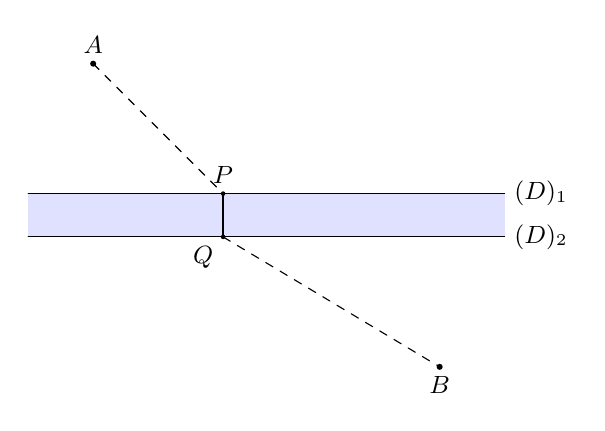
\begin{tikzpicture}[scale=0.55,line cap=round,>=stealth]
            \fill[blue!12] (-0.5,0) rectangle (10.5,1);
            \draw (-0.5,1) -- (10.5,1) node[right] {\small $\Droite_1$};
            \draw (-0.5,0) -- (10.5,0) node[right] {\small $\Droite_2$};
            \fill (1,4) circle (2pt) node[above] {\small $A$};
            \fill (9,-3) circle (2pt) node[below] {\small $B$};
            \draw[thick] (4,1) -- (4,0);
            \fill (4,1) circle (1.5pt) node[above] {\small $P$};
            \fill (4,0) circle (1.5pt) node[below left] {\small $Q$};
            \draw[dashed] (1,4) -- (4,1) (4,0) -- (9,-3);
      \end{tikzpicture}
      \end{center}
      \smallnota{La figure montre une position quelconque du pont, pas la position cherchée.}
\end{exo}
%%%%%%%%%%%%%%%%%%%%%%%%%%%%%%%%%%%%%%%%%%%%%%%%%%%%%%%%%%%%%%%%
\begin{exo}\label{exo:isom-napoleon}
      $ABC$ est un triangle quelconque du plan orienté. On note :
      \begin{itemize}
            \item $R$ le point tel que $RA = RB$ et $(\overrightarrow{RA},\overrightarrow{RB}) = \frac{2\pi}{3}\ [2\pi]$ ;
            \item $P$ le point tel que $PB = PC$ et $(\overrightarrow{PB},\overrightarrow{PC}) = \frac{2\pi}{3}\ [2\pi]$ ;
            \item $Q$ le point tel que $QC = QA$ et $(\overrightarrow{QC},\overrightarrow{QA}) = \frac{2\pi}{3}\ [2\pi]$ ;
      \end{itemize}
      et $r_R$, $r_P$, $r_Q$ les rotations d'angle $\frac{2\pi}{3}$ de centres respectifs $R$, $P$, $Q$.
      \begin{enumerate}
            \item Déterminer $r_R(A)$, $r_P(B)$ et $r_Q(C)$.
            \item Montrer que $r_Q \circ r_P \circ r_R$ est l'identité.
                  En déduire que $r_Q \circ r_P$ est la rotation de centre $R$ et d'angle $-\frac{2\pi}{3}$.
            \item On suppose dans cette question que $P \neq Q$.
                  Soit $X$ le point tel que le triangle $PQX$ soit équilatéral avec $(\overrightarrow{PQ},\overrightarrow{PX}) = -\frac{\pi}{3}\ [2\pi]$.
                  \begin{enumerate}
                        \item Montrer que $r_P = s_{(PQ)} \circ s_{(PX)}$ et $r_Q = s_{(QX)} \circ s_{(PQ)}$.
                        \item En déduire que $r_Q \circ r_P$ est une rotation de centre $X$.
                  \end{enumerate}
            \item Conclure que, si $P \neq Q$, le triangle $PQR$ est équilatéral.
                  Que dire de $R$ lorsque $P = Q$\,?
      \end{enumerate}
\end{exo}

\begin{corrige}
\section{Solutions des exercices}
%%%%%%%%%%%%%%%%%%%%%%%%%%%%%%%%%%%%%%%%%%%%%%%%%%%%%%%%%%%%%%%%
\begin{sol}[Exercice~\ref{exo:isom-analytique}]
\begin{enumerate}
      \item Les matrices sont
            $A_1 = \begin{pmatrix} 0 & -1 \\ 1 & 0 \end{pmatrix}$,
            $A_2 = \begin{pmatrix} 0 & 1 \\ 1 & 0 \end{pmatrix}$ et
            $A_3 = \begin{pmatrix} -1 & 0 \\ 0 & 1 \end{pmatrix}$.
            $A_1$ est du type $\begin{pmatrix} a & -b \\ b & a \end{pmatrix}$ avec $a = 0$, $b = 1$ ;
            $A_2$ et $A_3$ sont du type $\begin{pmatrix} a & b \\ b & -a \end{pmatrix}$ avec $(a,b) = (0,1)$ et $(a,b) = (-1,0)$.
            Dans chaque cas $a^2 + b^2 = 1$ : ce sont trois isométries.
            Les déterminants valent $\Delta_1 = 1$, $\Delta_2 = -1$, $\Delta_3 = -1$ :
            \fbox{$f_1$ est un déplacement, $f_2$ et $f_3$ sont des antidéplacements.}
      \item Avec $z = x + iy$ et $z' = x' + iy'$ :
            \begin{itemize}
                  \item $z' = (-y+3) + i(x+1) = i(x+iy) + 3 + i$, donc $f_1 : z' = iz + 3 + i$ ;
                  \item $z' = (y+1) + i(x-1) = i(x - iy) + 1 - i$, donc $f_2 : z' = i\bar{z} + 1 - i$ ;
                  \item $z' = (-x+4) + i(y+2) = -(x - iy) + 4 + 2i$, donc $f_3 : z' = -\bar{z} + 4 + 2i$.
            \end{itemize}
      \item $f_1$ : $a = i \neq 1$ et $|a| = 1$, donc $f_1$ est une rotation d'angle $\arg(i) = \frac{\pi}{2}$ et de centre
            $\Omega$ d'affixe $\frac{b}{1-a} = \frac{3+i}{1-i} = \frac{(3+i)(1+i)}{2} = \frac{2+4i}{2} = 1 + 2i$.
            \fbox{$f_1 = r\left(\Omega(1+2i),\frac{\pi}{2}\right)$.}

            $f_2$ : avec $a = i$, $b = 1 - i$, on a $a\bar{b} + b = i(1+i) + 1 - i = i - 1 + 1 - i = 0$ : $f_2$ est une réflexion.
            Ses points invariants vérifient $x = y + 1$ et $y = x - 1$ : \fbox{$f_2$ est la réflexion d'axe $y = x - 1$.}
      \item \begin{enumerate}
                  \item Un point invariant de $f_3$ vérifierait $x = -x + 4$ et $y = y + 2$ ; la seconde égalité est impossible :
                        $f_3$ n'a aucun point invariant (c'est donc une symétrie glissée).
                  \item $f_3 \circ f_3 : x'' = -(-x+4) + 4 = x$, $y'' = (y+2) + 2 = y + 4$ :
                        $f_3 \circ f_3$ est la translation de vecteur $(0;4)$.
                        Si $f_3 = t_{\vec{w}} \circ s_{\Droite}$ avec $\vec{w}$ directeur de $\Droite$, alors $t_{\vec{w}}$ et $s_{\Droite}$ commutent et
                        $f_3 \circ f_3 = t_{2\vec{w}}$, d'où $\vec{w}(0;2)$.
                        Alors $s_{\Droite} = t_{-\vec{w}} \circ f_3 : (x,y) \mapsto (-x + 4, y)$, dont les points invariants forment la droite
                        $x = 2$. \fbox{$f_3 = t_{\vec{w}} \circ s_{\Droite}$ avec $\vec{w}(0;2)$ et $\Droite : x = 2$.}
            \end{enumerate}
      \item $g(z) = f_2(iz + 3 + i) = i\,\overline{(iz + 3 + i)} + 1 - i = i(-i\bar{z} + 3 - i) + 1 - i = \bar{z} + 3i + 1 + 1 - i$,
            donc \fbox{$g : z' = \bar{z} + 2 + 2i$.}
            C'est un antidéplacement ; $a\bar{b} + b = (2 - 2i) + (2 + 2i) = 4 \neq 0$, donc $g$ n'est pas une réflexion : c'est une symétrie glissée.
            Analytiquement $x' = x + 2$, $y' = -y + 2$ : $g$ est la réflexion d'axe $y = 1$ (qui envoie $(x,y)$ sur $(x, 2-y)$)
            suivie de la translation de vecteur $(2;0)$, parallèle à cet axe.
            \fbox{Forme réduite : $g = t_{\vec{w}'} \circ s_{\Droite'}$, $\vec{w}'(2;0)$, $\Droite' : y = 1$.}
\end{enumerate}
\end{sol}
%%%%%%%%%%%%%%%%%%%%%%%%%%%%%%%%%%%%%%%%%%%%%%%%%%%%%%%%%%%%%%%%
\begin{sol}[Exercice~\ref{exo:isom-carre-reflexions}]
\begin{enumerate}
      \item Les droites $(AB)$ et $(DC)$ sont parallèles ; le projeté orthogonal de $A \in (AB)$ sur $(DC)$ est $D$. Donc
            \fbox{$s_{(DC)} \circ s_{(AB)} = t_{2\overrightarrow{AD}}$.}
            Les diagonales $(AC)$ et $(BD)$ se coupent en $O$ et sont perpendiculaires : $((AC),(BD)) = \frac{\pi}{2}\ [\pi]$, donc
            $s_{(BD)} \circ s_{(AC)} = r(O, \pi)$ : \fbox{c'est la symétrie de centre $O$.}
      \item \begin{enumerate}
                  \item $(AB)$ et $(AC)$ se coupent en $A$ et $((AB),(AC)) = \frac{\pi}{4}\ [\pi]$ (la diagonale est bissectrice de l'angle droit).
                        Donc $s_{(AC)} \circ s_{(AB)} = r\left(A, 2 \times \frac{\pi}{4}\right) = r_1$.
                  \item Il faut une droite $\Delta$ passant par $C$ telle que $((AC),\Delta) = \frac{\pi}{4}\ [\pi]$.
                        La droite $(CB)$ convient : $((AC),(CB)) = ((AC),(AD)) = \frac{\pi}{4}\ [\pi]$ car $(CB) \parallel (AD)$.
                        \fbox{$r_2 = s_{(CB)} \circ s_{(AC)}$.}
                  \item $r_2 \circ r_1 = s_{(CB)} \circ s_{(AC)} \circ s_{(AC)} \circ s_{(AB)} = s_{(CB)} \circ s_{(AB)}$ (car $s_{(AC)} \circ s_{(AC)} = \Id$).
                        Les droites $(AB)$ et $(CB)$ sont perpendiculaires en $B$, donc
                        \fbox{$r_2 \circ r_1$ est la symétrie de centre $B$.}
                        Vérification : $r_1(A) = A$ ; $r_2(A)$ est le point $A'$ tel que $CA' = CA$ et $(\overrightarrow{CA},\overrightarrow{CA'}) = \frac{\pi}{2}$.
                        Dans le repère $(A;\frac14\overrightarrow{AB},\frac14\overrightarrow{AD})$, $C(4;4)$, $\overrightarrow{CA}(-4;-4)$ tourné de $\frac{\pi}{2}$ donne $(4;-4)$,
                        d'où $A'(8;0)$ : c'est bien le symétrique de $A$ par rapport à $B(4;0)$.
            \end{enumerate}
      \item $r_1^{-1} = r(A,-\frac{\pi}{2})$. Comme $((AD),(AC)) = -\frac{\pi}{4}\ [\pi]$, on a $r_1^{-1} = s_{(AC)} \circ s_{(AD)}$.
            Alors $r_2 \circ r_1^{-1} = s_{(CB)} \circ s_{(AC)} \circ s_{(AC)} \circ s_{(AD)} = s_{(CB)} \circ s_{(AD)}$.
            Les droites $(AD)$ et $(CB)$ sont parallèles et le projeté de $A$ sur $(CB)$ est $B$ :
            \fbox{$r_2 \circ r_1^{-1} = t_{2\overrightarrow{AB}}$} (ce qui est cohérent avec la somme des angles $\frac{\pi}{2} - \frac{\pi}{2} = 0$).
\end{enumerate}
\end{sol}
%%%%%%%%%%%%%%%%%%%%%%%%%%%%%%%%%%%%%%%%%%%%%%%%%%%%%%%%%%%%%%%%
\begin{sol}[Exercice~\ref{exo:isom-rotation-translation}]
\begin{enumerate}
      \item La composée d'une rotation d'angle $\theta \neq 0\ [2\pi]$ et d'une translation (dans un ordre quelconque) est une rotation d'angle $\theta$ :
            $r \circ t$ et $t \circ r$ sont des rotations d'angle $\frac{\pi}{3}$.
      \item \begin{enumerate}
                  \item $\overrightarrow{C_1B_1} = \overrightarrow{C_1A} + \overrightarrow{AB_1} = \overrightarrow{AC} - \overrightarrow{AB} = \overrightarrow{BC}$,
                        donc $t(C_1) = B_1$.
                        La rotation $r$ transforme $B$ en $C$ (car $AB = AC$ et $(\overrightarrow{AB},\overrightarrow{AC}) = \frac{\pi}{3}$) ;
                        elle commute avec la symétrie de centre $A$ (rotation de même centre), donc $r(B_1) = C_1$.
                  \item $(r \circ t)(C_1) = r(B_1) = C_1$ : le point $C_1$ est invariant par la rotation $r \circ t$, c'en est le centre.
                        \fbox{$r \circ t = r\left(C_1, \frac{\pi}{3}\right)$.}
            \end{enumerate}
      \item $(t \circ r)(B_1) = t(C_1) = B_1$, donc \fbox{$t \circ r = r\left(B_1, \frac{\pi}{3}\right)$.}
      \item $\varphi$ est la composée d'une rotation d'angle $\frac{\pi}{3}$ et d'une rotation d'angle $-\frac{\pi}{3}$ : c'est une translation.
            $(r \circ t)^{-1}(C_1) = C_1$, donc $\varphi(C_1) = t(r(C_1))$.
            On a $\overrightarrow{A\,r(C)} = \overrightarrow{BC}$ (le triangle $AC\,r(C)$ est équilatéral direct, donc $ABC\,r(C)$ est un losange), puis
            $\overrightarrow{A\,r(C_1)} = -\overrightarrow{A\,r(C)} = \overrightarrow{CB}$, et enfin
            $\overrightarrow{A\,\varphi(C_1)} = \overrightarrow{CB} + \overrightarrow{BC} = \vec{0}$ : $\varphi(C_1) = A$.
            \fbox{$\varphi = t_{\overrightarrow{C_1A}} = t_{\overrightarrow{AC}}$.}
      \item Avec $\omega = e^{i\pi/3}$ : $z_A = 0$, $z_B = 1$, $z_C = \omega$, $z_{B_1} = -1$, $z_{C_1} = -\omega$ ;
            $r : z' = \omega z$ et $t : z' = z + \omega - 1$. On utilise $\omega^2 = \omega - 1$.
            \begin{itemize}
                  \item $r \circ t : z' = \omega(z + \omega - 1) = \omega z + \omega^2 - \omega = \omega z - 1$ ; centre $\frac{-1}{1-\omega} = \frac{-1}{e^{-i\pi/3}} = -\omega = z_{C_1}$.
                  \item $t \circ r : z' = \omega z + \omega - 1$ ; centre $\frac{\omega - 1}{1 - \omega} = -1 = z_{B_1}$.
                  \item $(r \circ t)^{-1} : z = \frac{z' + 1}{\omega}$, donc $\varphi : z' = \omega \cdot \frac{z+1}{\omega} + \omega - 1 = z + \omega$ :
                        translation de vecteur d'affixe $\omega = z_C$, c'est-à-dire $\overrightarrow{AC}$.
            \end{itemize}
\end{enumerate}
\end{sol}
%%%%%%%%%%%%%%%%%%%%%%%%%%%%%%%%%%%%%%%%%%%%%%%%%%%%%%%%%%%%%%%%
\begin{sol}[Exercice~\ref{exo:isom-symetrie-glissee}]
\begin{enumerate}
      \item $(EF)$ est l'image de $(AD)$ par $t_{\frac12\overrightarrow{AB}}$ et $\overrightarrow{AB}$ est orthogonal à $(AD)$, donc
            $t_{\overrightarrow{AB}} = s_{(EF)} \circ s_{(AD)}$. Ainsi $f = s_{(EF)} \circ s_{(AD)} \circ s_{(AD)} = s_{(EF)}$ :
            \fbox{$f$ est la réflexion d'axe $(EF)$, médiatrice de $[AB]$.}
      \item \begin{enumerate}
                  \item $(IJ)$ est l'image de $(AB)$ par $t_{\frac12\overrightarrow{AD}}$ et $\overrightarrow{AD} \perp (AB)$, donc
                        $t_{\overrightarrow{AD}} = s_{(IJ)} \circ s_{(AB)}$, d'où $t_{\overrightarrow{AD}} \circ s_{(AB)} = s_{(IJ)}$.
                  \item $\overrightarrow{AC} = \overrightarrow{AB} + \overrightarrow{AD}$, donc
                        $g = t_{\overrightarrow{AB}} \circ t_{\overrightarrow{AD}} \circ s_{(AB)} = t_{\overrightarrow{AB}} \circ s_{(IJ)}$.
                        Comme $\overrightarrow{AB}$ est un vecteur non nul qui dirige $(IJ)$,
                        \fbox{$g$ est une symétrie glissée d'axe $(IJ)$ et de vecteur $\overrightarrow{AB}$} : c'est sa forme réduite.
                  \item $s_{(IJ)}$ échange $A$ et $D$, $B$ et $C$. Donc $g(A) = t_{\overrightarrow{AB}}(D) = C$, $g(D) = t_{\overrightarrow{AB}}(A) = B$,
                        $g(B) = t_{\overrightarrow{AB}}(C) = K$ où $\overrightarrow{CK} = \overrightarrow{AB}$, et $g(C) = t_{\overrightarrow{AB}}(B) = L$,
                        symétrique de $A$ par rapport à $B$.
            \end{enumerate}
      \item \begin{enumerate}
                  \item $s_{(AB)} : z' = \bar{z}$ et $\overrightarrow{AC}$ a pour affixe $6 + 4i$, donc \fbox{$g : z' = \bar{z} + 6 + 4i$.}
                        Un point invariant vérifierait $x = x + 6$ : impossible.
                  \item Si $M(x;y)$, alors $M'(x+6; -y+4)$ et le milieu de $[MM']$ est $(x+3; 2)$, qui est sur $(IJ) : y = 2$.
            \end{enumerate}
\end{enumerate}
\end{sol}
%%%%%%%%%%%%%%%%%%%%%%%%%%%%%%%%%%%%%%%%%%%%%%%%%%%%%%%%%%%%%%%%
\begin{sol}[Exercice~\ref{exo:isom-deux-points}]
\begin{enumerate}
      \item $z_B - z_A = 2$ et $z_{B'} - z_{A'} = 2i$ : $AB = A'B' = 2$.
      \item \begin{enumerate}
                  \item $f : z' = az + b$ avec $a = \frac{z_{B'} - z_{A'}}{z_B - z_A} = \frac{2i}{2} = i$ et
                        $b = z_{A'} - a z_A = 2 + 3i - i(1+i) = 3 + 2i$. \fbox{$f : z' = iz + 3 + 2i$.}
                  \item $|a| = 1$, $a \neq 1$ : rotation d'angle $\frac{\pi}{2}$, de centre d'affixe
                        $\frac{3+2i}{1-i} = \frac{(3+2i)(1+i)}{2} = \frac{1 + 5i}{2}$.
            \end{enumerate}
      \item \begin{enumerate}
                  \item $g : z' = a\bar{z} + b$ avec $a = \frac{z_{B'} - z_{A'}}{\overline{z_B - z_A}} = \frac{2i}{2} = i$ et
                        $b = z_{A'} - a\,\overline{z_A} = 2 + 3i - i(1 - i) = 1 + 2i$. \fbox{$g : z' = i\bar{z} + 1 + 2i$.}
                        (Vérification : $g(3+i) = i(3 - i) + 1 + 2i = 2 + 5i$.)
                  \item Un antidéplacement est entièrement déterminé par les images de deux points distincts, donc $g$ est le seul antidéplacement qui convient.
                        Or $a\bar{b} + b = i(1 - 2i) + 1 + 2i = 3 + 3i \neq 0$ : $g$ n'est pas une réflexion.
                        \fbox{Aucune réflexion ne transforme $A$ en $A'$ et $B$ en $B'$.}
                  \item $g \circ g : z' = i\,\overline{(i\bar{z} + 1 + 2i)} + 1 + 2i = i(-iz + 1 - 2i) + 1 + 2i = z + 3 + 3i$.
                        Si $g = t_{\vec{w}} \circ s_{\Droite}$ ($\vec{w}$ directeur de $\Droite$), alors $g \circ g = t_{2\vec{w}}$, donc $\vec{w}$ a pour affixe $\frac{3+3i}{2}$.
                        L'axe est l'ensemble des points $M$ tels que $g(M) = t_{\vec{w}}(M)$ :
                        $i\bar{z} + 1 + 2i = z + \frac32 + \frac32 i$ s'écrit $y + 1 = x + \frac32$ et $x + 2 = y + \frac32$, soit $y = x + \frac12$ (les deux équations sont les mêmes).
                        \fbox{$g = t_{\vec{w}} \circ s_{\Droite}$, $\vec{w}\left(\frac32;\frac32\right)$, $\Droite : y = x + \frac12$} ($\vec{w}$ dirige bien $\Droite$).
            \end{enumerate}
\end{enumerate}
\end{sol}
%%%%%%%%%%%%%%%%%%%%%%%%%%%%%%%%%%%%%%%%%%%%%%%%%%%%%%%%%%%%%%%%
\begin{sol}[Exercice~\ref{exo:isom-deux-carres}]
\begin{enumerate}
      \item $AB = AD$ et $(\overrightarrow{AB},\overrightarrow{AD}) = \frac{\pi}{2}$, donc $r(B) = D$ ; de même $r(E) = G$.
            Une rotation conserve les distances : $DG = BE$. Elle tourne toute droite de son angle : $((BE),(DG)) = \frac{\pi}{2}\ [\pi]$,
            donc $(BE) \perp (DG)$.
      \item \begin{enumerate}
                  \item Dans le carré direct $ABCD$ de centre $O$, $OD = OA$ et $(\overrightarrow{OD},\overrightarrow{OA}) = \frac{\pi}{2}$ : $r_1(D) = A$.
                        De même dans $AEFG$ : $r_2(A) = E$.
                  \item $r_2 \circ r_1$ est un déplacement d'angle $\frac{\pi}{2} + \frac{\pi}{2} = \pi$ : c'est une symétrie centrale.
                        Elle envoie $D$ sur $r_2(A) = E$, donc son centre est le milieu $M$ de $[DE]$.
                  \item $O'O = O'O''$ et $(\overrightarrow{O'O},\overrightarrow{O'O''}) = \frac{\pi}{2}$ : le triangle $OO'O''$ est rectangle isocèle en $O'$.
                        De plus $r_1(O) = O$, donc $s_M(O) = r_2(r_1(O)) = r_2(O) = O''$ : $M$ est le milieu de $[OO'']$.
                  \item Dans le triangle $OO'O''$ rectangle isocèle en $O'$, la médiane $[O'M]$ est aussi hauteur, et $MO' = \frac12 OO'' = MO$.
                        Donc $(MO') \perp (MO)$ et $MO = MO'$ : \fbox{$OMO'$ est rectangle isocèle en $M$.}
            \end{enumerate}
\end{enumerate}
\end{sol}
%%%%%%%%%%%%%%%%%%%%%%%%%%%%%%%%%%%%%%%%%%%%%%%%%%%%%%%%%%%%%%%%
\begin{sol}[Exercice~\ref{exo:isom-triangle-invariant}]
\begin{enumerate}
      \item $O$ est l'isobarycentre de $A$, $B$, $C$. Une isométrie est une application affine, donc conserve les barycentres :
            $f(O)$ est l'isobarycentre de $f(A)$, $f(B)$, $f(C)$, c'est-à-dire de $A$, $B$, $C$ dans un autre ordre. Donc $f(O) = O$.
      \item Une application affine est déterminée par les images de trois points non alignés. Ici $(f(A),f(B),f(C))$ est une permutation de $(A,B,C)$,
            et il y a $3 \times 2 \times 1 = 6$ permutations : au plus six isométries.
      \item $O$ est le centre du cercle circonscrit et $(\overrightarrow{OA},\overrightarrow{OB}) = (\overrightarrow{OB},\overrightarrow{OC}) = (\overrightarrow{OC},\overrightarrow{OA}) = \frac{2\pi}{3}$ :
            $r(O,\frac{2\pi}{3})$ envoie $A \mapsto B \mapsto C \mapsto A$ et $r(O,-\frac{2\pi}{3})$ fait le tour inverse.
            $d_A$ passe par $A$ et est la médiatrice de $[BC]$ : $s_{d_A}$ fixe $A$ et échange $B$ et $C$ ; de même pour $s_{d_B}$ et $s_{d_C}$.
            Avec l'identité, cela fait six isométries distinctes qui conservent le triangle : ce sont toutes celles cherchées.
            \fbox{Trois déplacements ($\Id$ et les deux rotations) et trois antidéplacements (les trois réflexions).}
      \item $s_{d_A}(A) = A$ puis $s_{d_B}(A) = C$ : $s_{d_B} \circ s_{d_A}$ envoie $A$ sur $C$.
            C'est la composée de deux réflexions d'axes sécants en $O$, donc une rotation de centre $O$ ; comme elle envoie $A$ sur $C$,
            son angle est $(\overrightarrow{OA},\overrightarrow{OC}) = -\frac{2\pi}{3}$.
            Par les axes : $d_A = (OA)$ et $d_B = (OB)$, donc $(d_A,d_B) = (\overrightarrow{OA},\overrightarrow{OB}) = \frac{2\pi}{3}\ [\pi]$,
            et l'angle de la rotation est $2 \times \frac{2\pi}{3} = \frac{4\pi}{3} \equiv -\frac{2\pi}{3}\ [2\pi]$. \fbox{$s_{d_B} \circ s_{d_A} = r(O, -\frac{2\pi}{3})$.}
      \item C'est un antidéplacement qui conserve le triangle. $A \mapsto B \mapsto C$, $B \mapsto C \mapsto B$, $C \mapsto A \mapsto A$.
            Il fixe $B$ et $O$, échange $A$ et $C$ : \fbox{$s_{d_A} \circ r(O,\frac{2\pi}{3}) = s_{d_B}$.}
\end{enumerate}
\end{sol}
%%%%%%%%%%%%%%%%%%%%%%%%%%%%%%%%%%%%%%%%%%%%%%%%%%%%%%%%%%%%%%%%
\begin{sol}[Exercice~\ref{exo:isom-famille-antideplacements}]
\begin{enumerate}
      \item $f_m$ est de la forme $z' = a\bar{z} + b$ avec $a = i$, $|a| = 1$ : c'est un antidéplacement.
      \item $a\bar{b} + b = i(2 - mi) + 2 + mi = (m + 2) + (m+2)i = (m+2)(1+i)$.
            $f_m$ est une réflexion si et seulement si ce nombre est nul : \fbox{$m = -2$.}
            Alors $f_{-2} : z' = i\bar{z} + 2 - 2i$ ; les points invariants vérifient $x = y + 2$ et $y = x - 2$ :
            \fbox{axe $y = x - 2$.}
      \item \begin{enumerate}
                  \item $f_m \circ f_m : z' = i\,\overline{(i\bar{z} + b)} + b = i(-iz + \bar{b}) + b = z + i\bar{b} + b$, avec
                        $i\bar{b} + b = i(2 - mi) + 2 + mi = (m+2)(1+i)$. Donc $f_m \circ f_m = t_{\vec{v}}$ où $\vec{v}$ a pour affixe $(m+2)(1+i)$.
                  \item Pour $m \neq -2$, $f_m$ est un antidéplacement qui n'est pas une réflexion : c'est une symétrie glissée $t_{\vec{w}_m} \circ s_{\Droite_m}$
                        avec $\vec{w}_m$ directeur de $\Droite_m$, et $f_m \circ f_m = t_{2\vec{w}_m}$. D'où $z_{\vec{w}_m} = \frac{m+2}{2}(1+i)$.
                  \item $M \in \Droite_m \iff f_m(M) = t_{\vec{w}_m}(M)$ :
                        $y + 2 + i(x + m) = x + \frac{m+2}{2} + i\left(y + \frac{m+2}{2}\right)$, soit
                        $y = x + \frac{m+2}{2} - 2$ et $y = x + m - \frac{m+2}{2}$ ; ces deux équations sont identiques :
                        \fbox{$\Droite_m : y = x + \frac{m-2}{2}$.}
            \end{enumerate}
      \item Pour $m = -2$ la formule donne $y = x - 2$, l'axe trouvé en 2. Toutes les droites $\Droite_m$ ont pour coefficient directeur $1$ :
            elles sont parallèles à la première bissectrice.
\end{enumerate}
\end{sol}
%%%%%%%%%%%%%%%%%%%%%%%%%%%%%%%%%%%%%%%%%%%%%%%%%%%%%%%%%%%%%%%%
\begin{sol}[Exercice~\ref{exo:isom-plus-court-chemin}]
\begin{enumerate}
      \item \begin{enumerate}
                  \item $A_1(1;-3)$. La réflexion d'axe la route est une isométrie qui fixe $M$ et envoie $A$ sur $A_1$, donc $AM = A_1M$.
                        Par l'inégalité triangulaire, $A_1M + MB \geq A_1B$.
                  \item L'égalité a lieu si et seulement si $M \in [A_1B]$. $A_1$ et $B$ sont de part et d'autre de la route, donc $[A_1B]$ la coupe.
                        La droite $(A_1B)$ a pour coefficient directeur $\frac{1-(-3)}{7-1} = \frac23$ ; elle coupe l'axe des abscisses en
                        $x = 1 + \frac{3}{2/3} = \frac{11}{2}$. \fbox{$M\left(\frac{11}{2};0\right)$, trajet minimal $A_1B = \sqrt{36+16} = 2\sqrt{13} \approx 7{,}21~\mathrm{km}$.}
            \end{enumerate}
      \item \begin{enumerate}
                  \item $A_2 = t_{\vec{w}}(A)$ et $Q = t_{\vec{w}}(P)$ ; une translation conserve les distances, donc $AP = A_2Q$. On a $A_2(1;3)$.
                  \item Le trajet vaut $AP + PQ + QB = A_2Q + 1 + QB \geq A_2B + 1$, avec égalité si et seulement si $Q \in [A_2B]$
                        ($A_2$ et $B$ sont de part et d'autre de $\Droite_2$).
                        La droite $(A_2B)$ passe par $(1;3)$ avec le vecteur directeur $(8;-6)$ : elle coupe $y = 0$ pour $x = 1 + 8 \times \frac12 = 5$.
                        \fbox{Pont entre $P(5;1)$ et $Q(5;0)$ ; trajet minimal $A_2B + 1 = \sqrt{64 + 36} + 1 = 11~\mathrm{km}$.}
            \end{enumerate}
\end{enumerate}
\end{sol}
%%%%%%%%%%%%%%%%%%%%%%%%%%%%%%%%%%%%%%%%%%%%%%%%%%%%%%%%%%%%%%%%
\begin{sol}[Exercice~\ref{exo:isom-napoleon}]
\begin{enumerate}
      \item Par définition des points $R$, $P$, $Q$ : $r_R(A) = B$, $r_P(B) = C$, $r_Q(C) = A$.
      \item $r_Q \circ r_P \circ r_R$ est un déplacement d'angle $3 \times \frac{2\pi}{3} = 2\pi \equiv 0$ : c'est une translation.
            Elle envoie $A$ sur $r_Q(r_P(B)) = r_Q(C) = A$ : c'est la translation de vecteur nul, l'identité.
            En composant à droite par $r_R^{-1}$ : $r_Q \circ r_P = r_R^{-1} = r\left(R,-\frac{2\pi}{3}\right)$.
      \item \begin{enumerate}
                  \item Dans le triangle équilatéral $PQX$, $(\overrightarrow{PX},\overrightarrow{PQ}) = \frac{\pi}{3}$ et, l'orientation étant la même en chaque sommet,
                        $(\overrightarrow{QP},\overrightarrow{QX}) = \frac{\pi}{3}$.
                        Les droites $(PX)$ et $(PQ)$ se coupent en $P$ avec $((PX),(PQ)) = \frac{\pi}{3}\ [\pi]$, donc
                        $s_{(PQ)} \circ s_{(PX)} = r(P, \frac{2\pi}{3}) = r_P$.
                        De même $((PQ),(QX)) = \frac{\pi}{3}\ [\pi]$ et $s_{(QX)} \circ s_{(PQ)} = r(Q,\frac{2\pi}{3}) = r_Q$.
                  \item $r_Q \circ r_P = s_{(QX)} \circ s_{(PQ)} \circ s_{(PQ)} \circ s_{(PX)} = s_{(QX)} \circ s_{(PX)}$ : composée de deux réflexions
                        d'axes distincts sécants en $X$, c'est une rotation de centre $X$.
            \end{enumerate}
      \item Une rotation d'angle non nul a un seul point invariant, son centre. D'après 2 et 3, $X = R$ :
            \fbox{le triangle $PQR$ est équilatéral.}
            Si $P = Q$, alors $r_Q \circ r_P = r\left(P, \frac{4\pi}{3}\right) = r\left(P,-\frac{2\pi}{3}\right)$, donc $R = P$ : les trois points sont confondus
            (cela arrive par exemple pour un triangle équilatéral direct, où $P = Q = R$ est son centre).
\end{enumerate}
\end{sol}
\end{corrige}
